\chapter{Tab 4 · Control panel: control charts for predictive maintenance and quality control}\label{ch:panel}

\section{Idea}
Each run file contains far more than Cq values: the block temperature every 0.41\,s (.ixo instrument) or 1\,s (.eds instrument), the
exposure and lamp or LED values of every reading, the timing of the instrument's embedded computer and mechanics, and the
dates of every change. The control panel turns these numbers into \textbf{one history row per run} and draws
\textbf{58 control charts per instrument}, grouped in four families:

\begin{description}[leftmargin=2.6cm,style=nextline]
\item[1 · Hardware] thermal system, optics, mechanics — predictive maintenance;
\item[2 · Software] embedded computer, analysis software, data integrity;
\item[3 · Method] reagents, probes, assay behaviour;
\item[4 · Operator] pipetting precision, contamination, unadjusted comparisons (funnel plots).
\end{description}

Charts compare an instrument only with itself. Each tile shows a status light for the latest run (green in control, amber
watch, red alarm, grey not enough data), the latest value and a sparkline; a click opens the chart page.

\figui[0.82]{ui_panel_lc1.png}{Control panel for the synthetic .ixo instrument \texttt{LC-DEMO-01} (180 runs: 150 imported history rows and 30 runs built in the page). Summary cards, then the tiles of the hardware, software, method and operator groups.}{ui_panel_lc1}

{\footnotesize
\begin{longtable}{@{}lllll@{}}
\toprule \textbf{Code} & \textbf{Chart} & \textbf{Instr.} & \textbf{Default} & \textbf{Unit} \\\midrule\endfirsthead
\toprule \textbf{Code} & \textbf{Chart} & \textbf{Instr.} & \textbf{Default} & \textbf{Unit} \\\midrule\endhead
\texttt{B-H1} & Peak heating rate (2-s window) & LC QS & Trend & °C/s \\\hline
\texttt{B-H2} & Peak cooling rate (2-s window) & LC QS & Trend & °C/s \\\hline
\texttt{B-H3} & Overshoot at the denaturation step & LC QS & CUSUM & °C \\\hline
\texttt{B-H3b} & Settling time at the denaturation step & LC QS & I-MR & s \\\hline
\texttt{B-H3c} & Transition time A → B °C & LC QS & I-MR & s \\\hline
\texttt{B-H4} & Temperature at the moment of reading & LC QS & X̄–S & °C from setpoint \\\hline
\texttt{B-H5} & Block zone uniformity (95th percentile) & QS & EWMA & °C \\\hline
\texttt{B-H6} & Heat-sink maximum & QS & I-MR & °C \\\hline
\texttt{B-H6b} & Heated cover temperature & QS & I-MR & °C \\\hline
\texttt{B-H8} & Lamp reference channel (stability) & LC & I-MR & reference counts \\\hline
\texttt{B-H9} & Lamp drift within a run & LC & I-MR & \% change in the run \\\hline
\texttt{B-H10} & LED drive current & QS & Trend & current (as logged) \\\hline
\texttt{B-H10b} & LED junction temperature (maximum) & QS & I-MR & °C \\\hline
\texttt{B-H11} & Automatic integration time / exposure & LC QS & I-MR & ms \\\hline
\texttt{B-H12} & Saturated well images & QS & p & share of well images \\\hline
\texttt{B-H13} & Uniformity calibration: edge-to-centre ratio & QS & I-MR & edge / centre \\\hline
\texttt{B-H13b} & Background calibration: mean offset & QS & I-MR & counts \\\hline
\texttt{B-H13c} & Well-position (ROI) calibration: spot diameter & QS & I-MR & pixels \\\hline
\texttt{B-H14} & Filter-wheel move time & QS & I-MR & ms \\\hline
\texttt{B-H14b} & Filter-wheel moves slower than 500 ms & QS & p & share of moves \\\hline
\texttt{B-H15} & Filter-wheel position offset & QS & I-MR & encoder counts \\\hline
\texttt{B-H16} & Camera readout time beyond the exposure & QS & X̄–S & ms \\\hline
\texttt{B-H17} & Channel switch time & LC & I-MR & ms \\\hline
\texttt{B-H18} & Heated cover lowering time & QS & Trend & s \\\hline
\texttt{B-H18b} & Heated cover raising time & QS & I-MR & s \\\hline
\texttt{A-H3} & Background fluorescence per channel & LC QS & I-MR & fluorescence \\\hline
\texttt{A-H3b} & End-point fluorescence per channel & LC QS & I-MR & fluorescence \\\hline
\texttt{A-H4} & Run duration & LC QS & I-MR & minutes \\\hline
\texttt{B-S1} & Reply time to the PC software & QS & I-MR & ms (95th pct) \\\hline
\texttt{B-S2} & Once-per-second timer lateness & QS & I-MR & ms (95th pct) \\\hline
\texttt{B-S2b} & Scheduler falling behind & QS & u & events per run hour \\\hline
\texttt{B-S3} & Image → processing delay & QS & I-MR & ms (95th pct) \\\hline
\texttt{B-S4} & Image analysis time & QS & I-MR & ms \\\hline
\texttt{B-S5} & Run-time prediction error & QS & I-MR & \% \\\hline
\texttt{B-S6} & Data hand-off time & QS & I-MR & minutes \\\hline
\texttt{B-S8} & Command errors in the instrument log & QS & c & errors \\\hline
\texttt{B-S9} & Cycle-timing regularity & LC QS & I-MR & ms \\\hline
\texttt{B-S10} & Temperature-log intervals over 500 ms & LC & p & share of intervals \\\hline
\texttt{B-S11} & Invalid fluorescence readings & LC & p & share of readings \\\hline
\texttt{B-S12} & Stored Ct not reproducible (> 0.2) & QS & p & share of wells \\\hline
\texttt{A-S4} & Run end → last change & LC QS & I-MR & log10 hours \\\hline
\texttt{A-S6} & Forensic findings per run & LC QS & c & findings \\\hline
\texttt{A-M1} & Positive control Cq (Levey-Jennings) & LC QS & I-MR & Cq \\\hline
\texttt{B-M1} & Probe signal strength (positive control) & LC QS & EWMA & fluorescence \\\hline
\texttt{B-M2} & Passive reference (ROX) level & QS & I-MR & passive reference \\\hline
\texttt{B-M3} & PCR efficiency from the standards & LC QS & Trend & \% efficiency \\\hline
\texttt{B-M5} & Negative controls by process stage & LC QS & p & share of NTC wells \\\hline
\texttt{B-M6} & IC shift from fixed reference & LC QS & EWMA & cycles \\\hline
\texttt{B-M9} & Low Cq confidence & QS & p & share of wells \\\hline
\texttt{B-M10} & Late signal / stochastic-zone results & LC QS & p & share of results \\\hline
\texttt{B-O1} & Replicate precision (pooled SD, Cq < 30) & LC QS & I-MR & Cq SD \\\hline
\texttt{B-O2} & Dispensed-volume spread (ROX CV) & QS & I-MR & \% CV \\\hline
\texttt{B-O3} & Row / column pattern & LC QS & I-MR & Cq \\\hline
\texttt{B-O5} & Contamination rate by operator (funnel) & LC QS & Funnel & share of NTC wells \\\hline
\texttt{B-O6} & Repeat / inconclusive / invalid rate by operator … & LC QS & Funnel & share of results \\\hline
\texttt{B-O7} & Manual interventions & LC QS & p & share of settings \\\hline
\texttt{B-O9} & Stored calls that disagree with the SOP & LC QS & p & share of wells \\\hline
\texttt{B-O11} & Copied-data events & LC QS & c & events \\\hline
\bottomrule
\end{longtable}}



\section{History rows}
A history row holds everything a chart needs, a few kilobytes per run, so years of runs fit in one JSON file that the
laboratory keeps and re-imports. The key of a row is the SHA-256 of the source file, so the same file is never counted twice.
Hardware and software numbers (\texttt{ccStatic}) are fixed when the file is read; method and operator numbers
(\texttt{ccDynamic}) follow the SOP profile and are recomputed when it changes.

\begin{lstlisting}[style=vstyle,language=json, numbers=left,firstnumber=1]
{ "schema": "qpcr-instrument-history/1", "note": "SYNTHETIC demonstration history — all values are made up",
  "rows": [ { "key": "demo-hist-LC1-0042", "run": "DEMO_LC1_HIST_0043", "platform": "LC",
      "instrument": "LC · LC-DEMO-01", "date": 1718784000000, "operator": "Analyst C",
      "software": "LCS480 1.5.1.62", "firmware": "HTC_VER_10",
      "protocol": "95/600s@4.4 95/15s@4.4 60/60s@2.2 72/1s@4.4 40/30s@2.2",
      "m": { "heat_rate": 4.89, "cool_rate": 2.43, "settling": 6.15,
             "transition": {"95→60 °C": 14.66, "60→72 °C": 2.30, "72→95 °C": 5.74},
             "hold_temp": {"mean": -0.50, "sd": 0.031, "n": 45},
             "ntc_rate": {"extraction blank": {"bad": 1, "n": 6}}, "…": "…" } } ] }
\end{lstlisting}

\par\medskip\noindent{\small\textbf{Listing}~\texttt{ccRowsFromRuns()}\hfill\textcolor{gray}{HTML lines 6332--6346}}\par\nopagebreak
\lstinputlisting[style=vstyle,language=JavaScript,firstnumber=6332]{code/ccRowsFromRuns.js}


\par\medskip\noindent{\small\textbf{Listing}~\texttt{ccStatic()}\hfill\textcolor{gray}{HTML lines 5782--5848}}\par\nopagebreak
\lstinputlisting[style=vstyle,language=JavaScript,firstnumber=5782]{code/ccStatic.js}


\par\medskip\noindent{\small\textbf{Listing}~\texttt{ccDynamic()}\hfill\textcolor{gray}{HTML lines 5850--5899}}\par\nopagebreak
\lstinputlisting[style=vstyle,language=JavaScript,firstnumber=5850]{code/ccDynamic.js}


\par\medskip\noindent{\small\textbf{Listing}~\texttt{ccRowsFor()}\hfill\textcolor{gray}{HTML lines 6352--6357}}\par\nopagebreak
\lstinputlisting[style=vstyle,language=JavaScript,firstnumber=6352]{code/ccRowsFor.js}


\par\medskip\noindent{\small\textbf{Listing}~\texttt{ccImport()}\hfill\textcolor{gray}{HTML lines 6765--6773}}\par\nopagebreak
\lstinputlisting[style=vstyle,language=JavaScript,firstnumber=6765]{code/ccImport.js}


\par\medskip\noindent{\small\textbf{Listing}~\texttt{ccHistoryJSON()}\hfill\textcolor{gray}{HTML lines 6739--6743}}\par\nopagebreak
\lstinputlisting[style=vstyle,language=JavaScript,firstnumber=6739]{code/ccHistoryJSON.js}



\section{Instrument numbers from the temperature log}

\subsection*{Program fingerprint}
Thermal numbers are comparable only between runs of the same program. Every run gets a fingerprint
(\texttt{target/hold@ramp} per segment) and the panel can be restricted to one program.

\par\medskip\noindent{\small\textbf{Listing}~\texttt{ccSetpoints()}\hfill\textcolor{gray}{HTML lines 5706--5709}}\par\nopagebreak
\lstinputlisting[style=vstyle,language=JavaScript,firstnumber=5706]{code/ccSetpoints.js}


\par\medskip\noindent{\small\textbf{Listing}~\texttt{ccProtocolKey()}\hfill\textcolor{gray}{HTML lines 5924--5927}}\par\nopagebreak
\lstinputlisting[style=vstyle,language=JavaScript,firstnumber=5924]{code/ccProtocolKey.js}



\subsection*{Peak ramp rates, overshoot and settling}
The steepest 2-second slope of each transition, median over the run, is independent of plateau detection.
\texttt{ccThermalSteps()} finds the plateaus at the programmed setpoints and measures overshoot and settling time
(from the 90\,\% point until the block stays within $\pm0.5$\,°C).

\par\medskip\noindent{\small\textbf{Listing}~\texttt{ccPeakRates()}\hfill\textcolor{gray}{HTML lines 5684--5696}}\par\nopagebreak
\lstinputlisting[style=vstyle,language=JavaScript,firstnumber=5684]{code/ccPeakRates.js}


\par\medskip\noindent{\small\textbf{Listing}~\texttt{ccThermalSteps()}\hfill\textcolor{gray}{HTML lines 5595--5627}}\par\nopagebreak
\lstinputlisting[style=vstyle,language=JavaScript,firstnumber=5595]{code/ccThermalSteps.js}


\par\medskip\noindent{\small\textbf{Listing}~\texttt{ccThermalSummary()}\hfill\textcolor{gray}{HTML lines 5697--5705}}\par\nopagebreak
\lstinputlisting[style=vstyle,language=JavaScript,firstnumber=5697]{code/ccThermalSummary.js}



\subsection*{Transition time A $\to$ B}
The time from leaving $\pm0.5$\,°C of the start temperature until the block is within $\pm0.5$\,°C of the target, for every
transition the program asks for. Band crossings are interpolated between samples (at 4.4\,°C/s the .ixo instrument moves about
1.8\,°C between two samples, more than the band); passing through another setpoint is ignored, and a hold of at least 2\,s at a
temperature that is not the next step resets the starting point.

\par\medskip\noindent{\small\textbf{Listing}~\texttt{ccTransitionPairs()}\hfill\textcolor{gray}{HTML lines 5635--5646}}\par\nopagebreak
\lstinputlisting[style=vstyle,language=JavaScript,firstnumber=5635]{code/ccTransitionPairs.js}


\par\medskip\noindent{\small\textbf{Listing}~\texttt{ccTransitions()}\hfill\textcolor{gray}{HTML lines 5647--5673}}\par\nopagebreak
\lstinputlisting[style=vstyle,language=JavaScript,firstnumber=5647]{code/ccTransitions.js}


\par\medskip\noindent{\small\textbf{Listing}~\texttt{ccThin()}\hfill\textcolor{gray}{HTML lines 5676--5683}}\par\nopagebreak
\lstinputlisting[style=vstyle,language=JavaScript,firstnumber=5676]{code/ccThin.js}



\section{Statistics}\label{sec:stats}
All limits come from a \textbf{baseline} (Phase~I): the first $n$ runs (default 20; the full configured baseline is required before statistical alarms), or the runs from a
\emph{baseline start date} onwards (after a service). Runs before that date are drawn grey without limits.

\par\medskip\noindent{\small\textbf{Listing}~\texttt{ccPhase()}\hfill\textcolor{gray}{HTML lines 6143--6143}}\par\nopagebreak
\lstinputlisting[style=vstyle,language=JavaScript,firstnumber=6143]{code/ccPhase.js}



\subsection{Individuals chart (I-MR) and run rules}
With $\bar x$ the baseline mean and $\overline{MR}$ the mean moving range,
\[ \hat\sigma=\max\!\Big(\frac{\overline{MR}}{1.128},\ \frac{r}{2}\Big),\qquad \text{limits } \bar x\pm3\hat\sigma , \]
where $r$ is the measurement resolution of quantised values (0.41\,s log samples, 10\,ms channel switch), so a baseline of
identical values does not give $\hat\sigma=0$. Western Electric rules 2--5 (2 of 3 beyond $2\sigma$, 4 of 5 beyond $1\sigma$,
8 on one side, 6 rising or falling) are switchable per chart.

\par\medskip\noindent{\small\textbf{Listing}~\texttt{ccI()}\hfill\textcolor{gray}{HTML lines 6145--6157}}\par\nopagebreak
\lstinputlisting[style=vstyle,language=JavaScript,firstnumber=6145]{code/ccI.js}



\fig[0.9]{cc_wheel_ms.png}{I chart, .eds instrument \texttt{QS-DEMO-A}, B-H14 filter-wheel move time. The planted step of +14\,ms from 2025-09 puts every later run outside the old limits; the page reports it as one sustained shift (Section~\ref{sec:shift}) instead of an alarm per run.}{wheel}
\fig[0.9]{cc_settling.png}{I chart with resolution floor, B-H3b settling time. The value moves in whole log samples (0.41\,s); the planted service step shortens it by one sample, which is the 3$\sigma$ signal, while values on the centre line raise no pattern rule.}{settling}

\subsection{Signal classes: outside the limits versus a pattern inside them}\label{sec:signals}
A flag is not evidence of the same kind in every case. The page separates two classes, computed from the flag text by
\texttt{ccSignal()}:
\begin{itemize}
\item \textbf{limit signal} — the point itself lies outside a control limit or a specification (beyond $3\sigma$, $1_{3s}$,
      off the trend band, EWMA or CUSUM alarm, above a $p$/$u$/$c$ limit, outside the specification). Drawn \textbf{red};
\item \textbf{rule signal} — the point is inside the limits and belongs to a suspicious pattern (Western Electric 2--5,
      Westgard $2_{2s}$, $4_{1s}$, $10_{\bar x}$). Drawn \textbf{amber}.
\end{itemize}
The tile status is red only for a limit signal, or for a pattern rule on a control material (Westgard charts); a pattern on an
equipment chart gives ``watch''. Tooltips read \emph{outside the limits} or \emph{pattern inside the limits}, and the CSV of
every chart carries a \texttt{signal} column with the class.

\par\medskip\noindent{\small\textbf{Listing}~\texttt{ccSignal()}\hfill\textcolor{gray}{HTML lines 5968--5969}}\par\nopagebreak
\lstinputlisting[style=vstyle,language=JavaScript,firstnumber=5968]{code/ccSignal.js}



Two further rules keep the pattern tests honest:
\begin{itemize}
\item a value that falls on the centre line is on \emph{no} side, so runs of identical values no longer produce ``8 on one
      side'' or $10_{\bar x}$;
\item for quantised series a value closer to the centre than half the resolution step ($r/2$; 0.41\,s for the temperature log)
      counts as on the centre, because it cannot be distinguished from it. The $3\sigma$ test is unchanged (Listing \texttt{ccI()}).
\end{itemize}

Background, plateau, exposure, run length, edit delay, lamp drift and cycle timing follow the plate that was run, not the
instrument. Sustained patterns there mirror the work schedule, so rules 2--5 are off by default for those charts and can be
switched on per chart in the settings.

\par\medskip\noindent{\small\textbf{Listing}~\texttt{CC\_RULES\_OFF, ccCfg()}\hfill\textcolor{gray}{HTML lines 6134--6135}}\par\nopagebreak
\lstinputlisting[style=vstyle,language=JavaScript,firstnumber=6134]{code/ccRulesOff.js}



\begin{figure}[htbp]\centering
\begin{subfigure}{0.49\linewidth}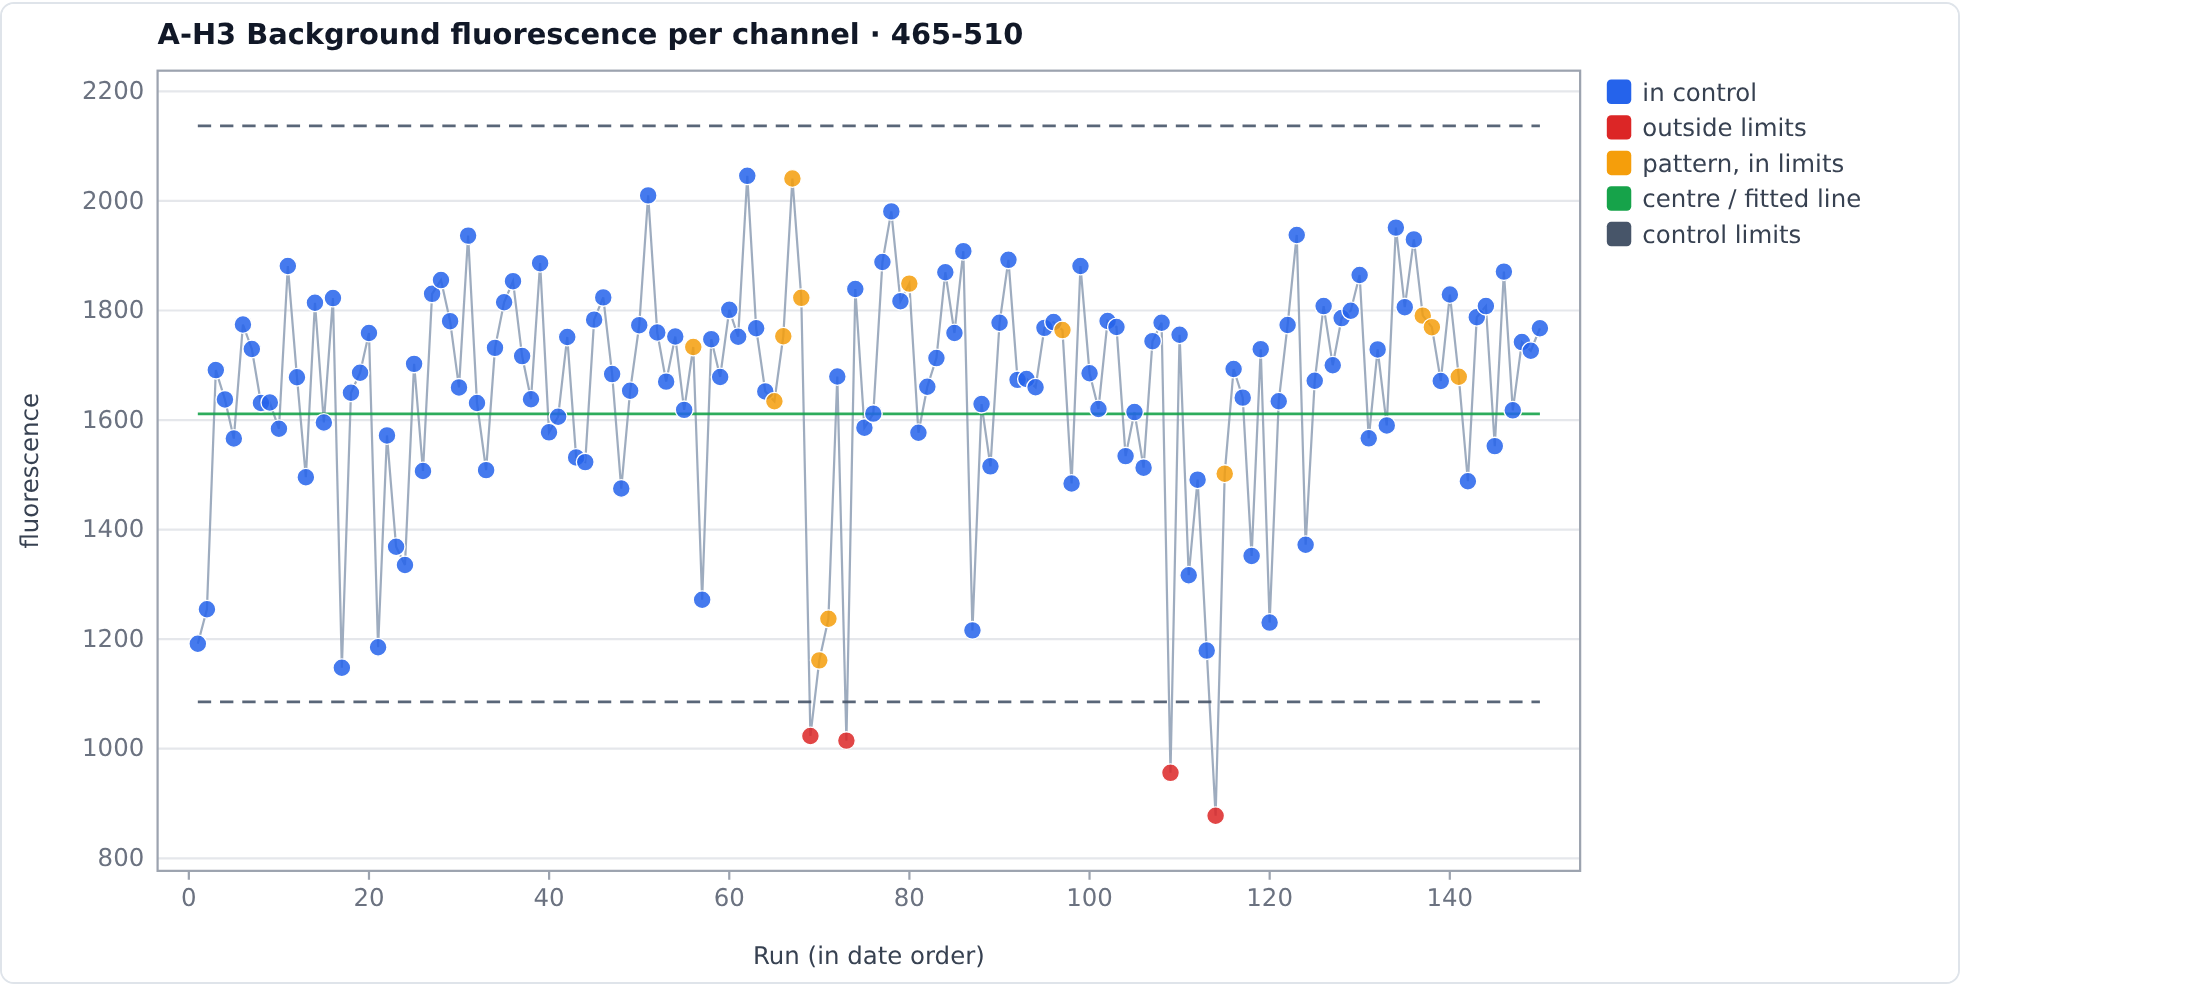
\includegraphics[width=\linewidth]{fig/cc_bg_signal_classes.png}\caption{pattern rules switched on}\label{fig:sig_on}\end{subfigure}\hfill
\begin{subfigure}{0.49\linewidth}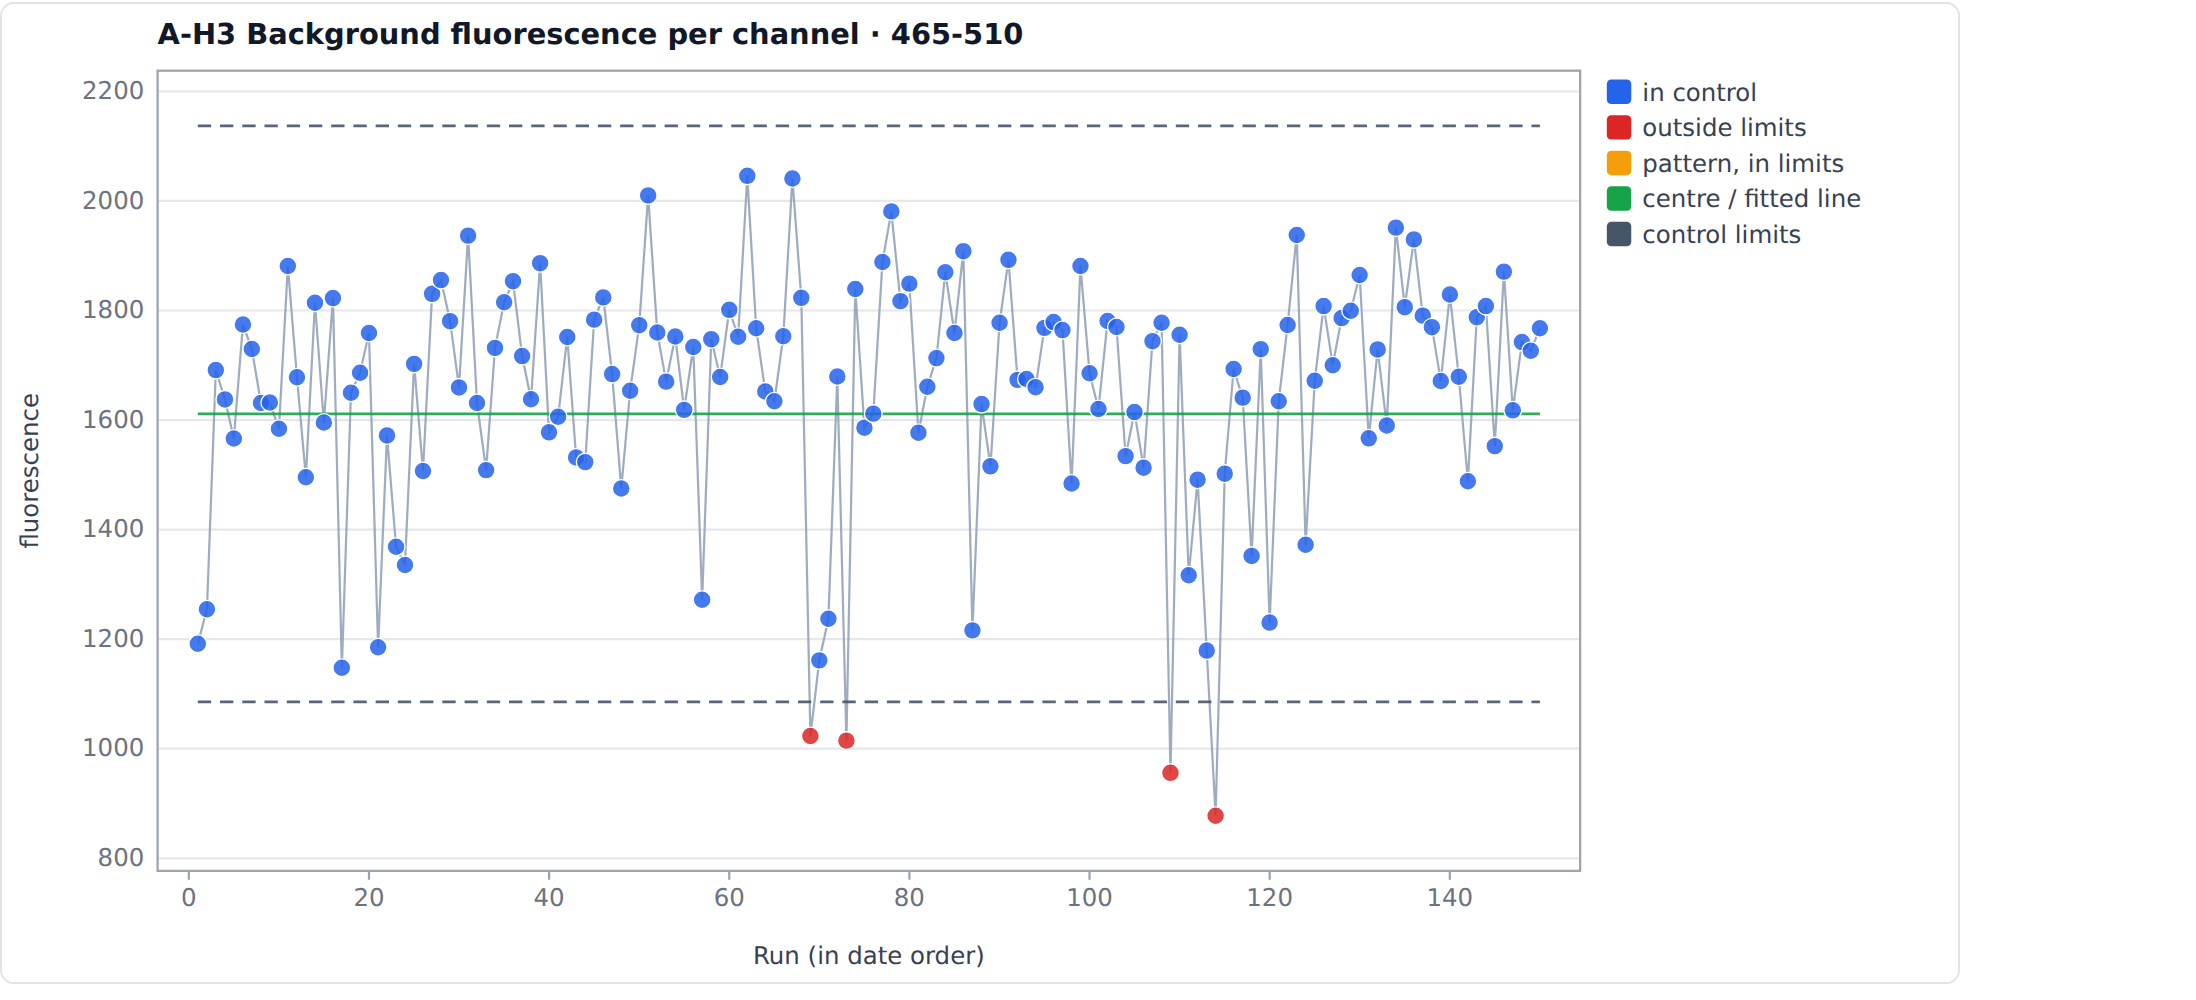
\includegraphics[width=\linewidth]{fig/cc_bg_rules_off.png}\caption{default: only the $3\sigma$ rule}\label{fig:sig_off}\end{subfigure}
\caption{\synthtag A-H3 background fluorescence, LC-DEMO-01, 465-510. In (a) the amber points are inside the control limits and
come from pattern rules; only the four red points are outside a limit. (b) is the default view of the same data.}\label{fig:signals}
\end{figure}
\readingnote{Red asks what happened in that run; amber asks whether the recent plates differ from the baseline period.}

\subsection{Levey-Jennings with Westgard rules}
Control materials use the Westgard multirule on the individuals chart: $1_{3s}$, $2_{2s}$, $4_{1s}$, $10_{\bar x}$. The across-run $R_{4s}$ rule has been removed; it requires a suitable within-run design.
\par\medskip\noindent{\small\textbf{Listing}~\texttt{ccWestgard()}\hfill\textcolor{gray}{HTML lines 6159--6169}}\par\nopagebreak
\lstinputlisting[style=vstyle,language=JavaScript,firstnumber=6159]{code/ccWestgard.js}


\fig[0.9]{cc_pc_cq_35S.png}{A-M1 positive-control Cq, 35S on the demonstration CRM. Each synthetic extract has its own baseline and limits (Section~\ref{sec:extracts}).}{pccq}

\subsection{Control materials: one series per target and material, one segment per extract}\label{sec:extracts}
A positive control is identified by target \emph{and} material (\texttt{35S | 415B}); the extract — extraction date plus any
aliquot or dilution qualifier — is kept separately and becomes a \textbf{segment} of the same chart. Each extract carries its
own baseline and limits, because a new extract is a new process; an extract with fewer runs than the baseline shows no limits
and the tile says how many runs are still missing. Target aliases (\texttt{P35S}/\texttt{35S}, \texttt{TNOS}/\texttt{T-NOS},
\texttt{hmgA}/\texttt{HMG}, \texttt{Le1}/\texttt{LEC}) are merged, and an extraction date later than the run is labelled
\emph{after run} rather than corrected. Histories written before this change are converted on import.

\par\medskip\noindent{\small\textbf{Listing}~\texttt{ccMigrateControlKeys()}\hfill\textcolor{gray}{HTML lines 6370--6382}}\par\nopagebreak
\lstinputlisting[style=vstyle,language=JavaScript,firstnumber=6370]{code/ccMigrate.js}



\fig[0.9]{cc_pc_extract_segments.png}{A-M1 positive-control Cq, one series (35S, demonstration CRM) with two synthetic extracts.
Each extract has its own centre line and limits in its own colour; the dotted line is the first run of the second extract.}{pcseg}
\readingnote{Comparing across the boundary answers a different question (did the material change?) from comparing inside one
segment (is the assay stable?). The chart keeps them apart.}

\subsection{EWMA}
\[ z_i=\lambda x_i+(1-\lambda)z_{i-1},\qquad \bar x\pm L\hat\sigma\sqrt{\tfrac{\lambda}{2-\lambda}\big(1-(1-\lambda)^{2i}\big)},\quad \lambda=0.2,\ L=2.7 . \]
\par\medskip\noindent{\small\textbf{Listing}~\texttt{ccEWMA()}\hfill\textcolor{gray}{HTML lines 6170--6175}}\par\nopagebreak
\lstinputlisting[style=vstyle,language=JavaScript,firstnumber=6170]{code/ccEWMA.js}


\fig[0.9]{cc_zone_spread_ewma.png}{EWMA, QS-DEMO-A, B-H5 block zone uniformity: the slow planted drift crosses the EWMA limit long before single values look unusual.}{ewma}

\subsection{CUSUM}
With $z_i=(x_i-\bar x)/\hat\sigma$: $C^+_i=\max(0,C^+_{i-1}+z_i-k)$, $C^-_i=\max(0,C^-_{i-1}-z_i-k)$, alarm when either exceeds $h$ ($k=0.5$, $h=4$).
\par\medskip\noindent{\small\textbf{Listing}~\texttt{ccCUSUM()}\hfill\textcolor{gray}{HTML lines 6176--6191}}\par\nopagebreak
\lstinputlisting[style=vstyle,language=JavaScript,firstnumber=6176]{code/ccCUSUM.js}


\fig[0.9]{cc_overshoot_cusum.png}{CUSUM, LC-DEMO-01, B-H3 overshoot at the denaturation step. In the calibrated demonstration data the overshoot is not changed by the planted service, and both sums stay below $h=4$: this is what an in-control CUSUM looks like.}{cusum}

\subsection{Trend (wear) chart with prediction}
After Oprime et al.\ (2025): a least-squares line $\hat y=a+bx$ is fitted to Phase~I by default (an explicit setting permits all runs since the baseline),
the limits follow the line at $\pm3s$ ($s$ = residual SD), and the crossing of the line with the specification limit gives the
forecast ``limit in $\approx N$ runs''. The tile turns amber when $N$ is below the \emph{warn ahead} setting. A slope that is
not significant on the baseline ($|t|=|b|/\mathrm{SE}(b)<2$) is not carried forward: the centre line is then flat, so noise in a
short baseline cannot turn every later run into a departure from a fitted trend. The projection is drawn at most 35\,\% beyond
the span of the data; if the limit lies further away the chart says so in words instead of stretching the axis.
\par\medskip\noindent{\small\textbf{Listing}~\texttt{ccTrend()}\hfill\textcolor{gray}{HTML lines 6193--6208}}\par\nopagebreak
\lstinputlisting[style=vstyle,language=JavaScript,firstnumber=6193]{code/ccTrend.js}



\begin{figure}[htbp]\centering
\begin{subfigure}{0.49\linewidth}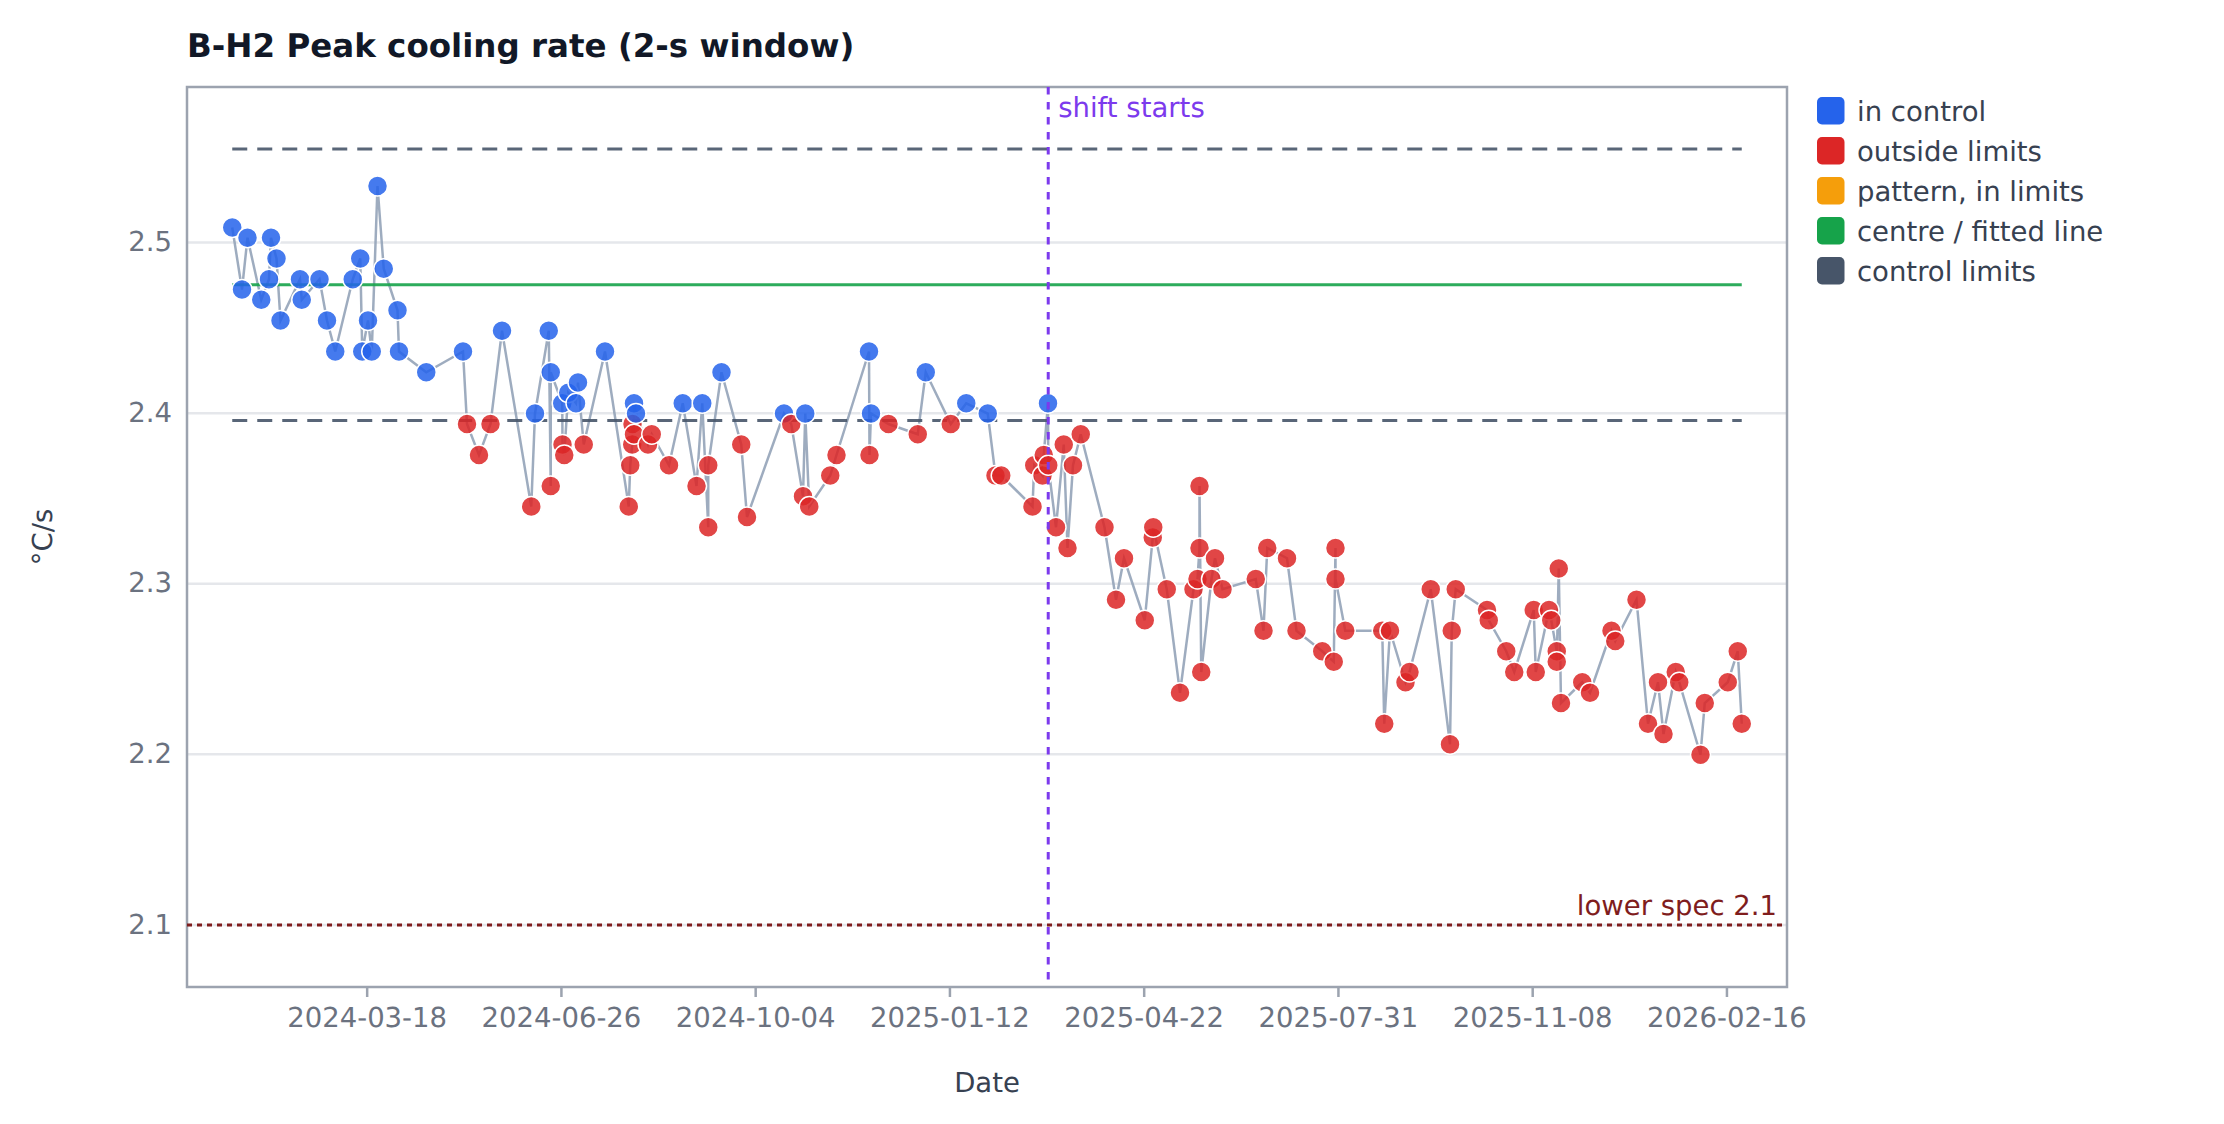
\includegraphics[width=\linewidth]{fig/cc_cool_rate_before.png}\caption{fixed Phase-I fit}\label{fig:cool_before}\end{subfigure}\hfill
\begin{subfigure}{0.49\linewidth}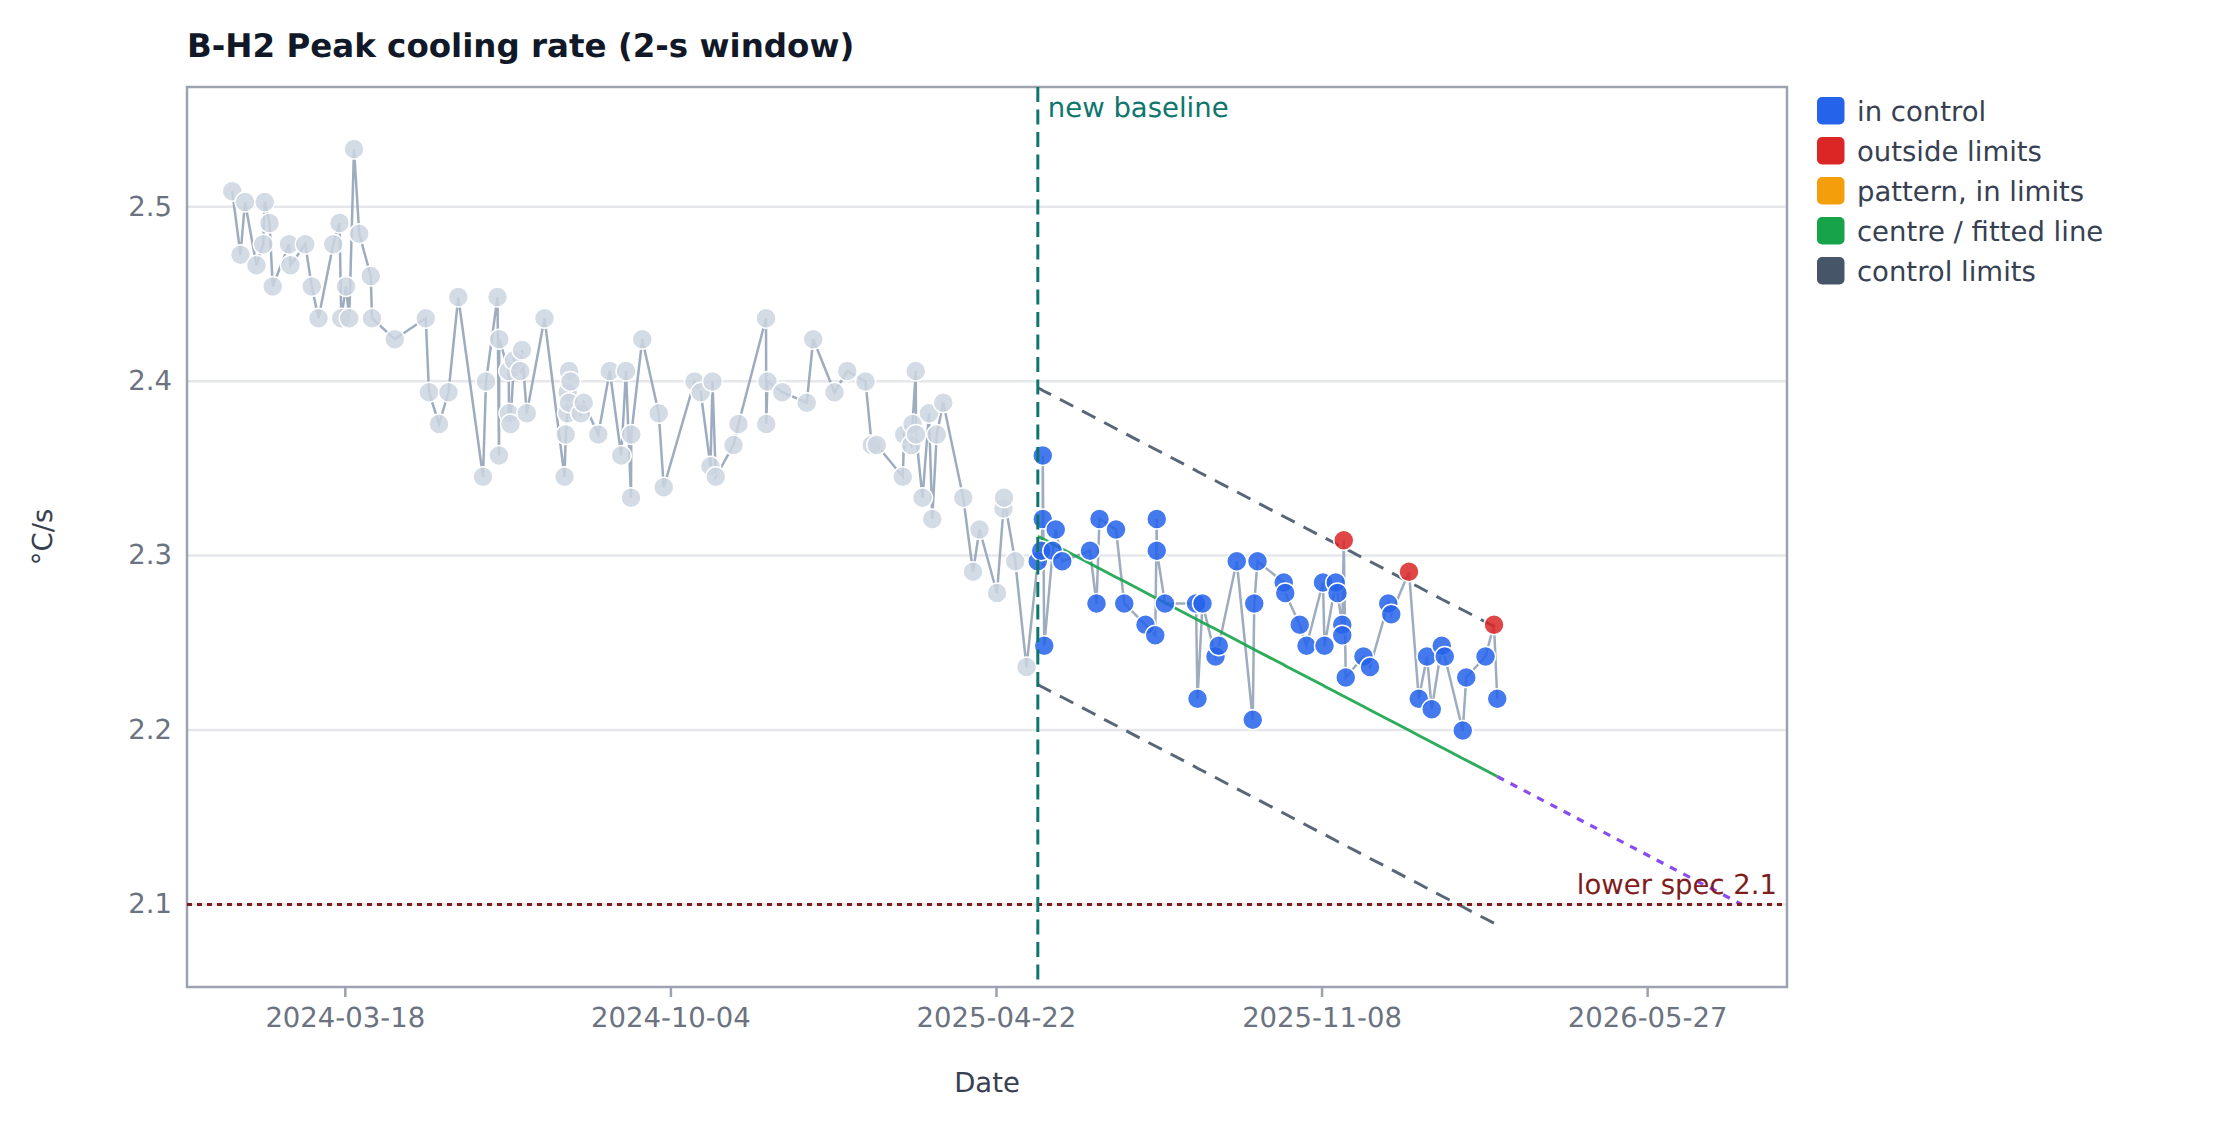
\includegraphics[width=\linewidth]{fig/cc_cool_rate_rebaseline.png}\caption{baseline from the service date}\label{fig:cool_rebase}\end{subfigure}
\caption{\synthtag Trend chart, LC-DEMO-01, B-H2 peak cooling rate against date. (a) The baseline precedes the planted service step.
(b) With \emph{Baseline starts on} = 2025-05-12 the earlier runs are grey, a green marker shows the new baseline and the
fit uses the configured Phase-I runs after service. Forecasts depend on this selection and are illustrative.}\label{fig:cool}
\end{figure}

\begin{figure}[htbp]\centering
\begin{subfigure}{0.49\linewidth}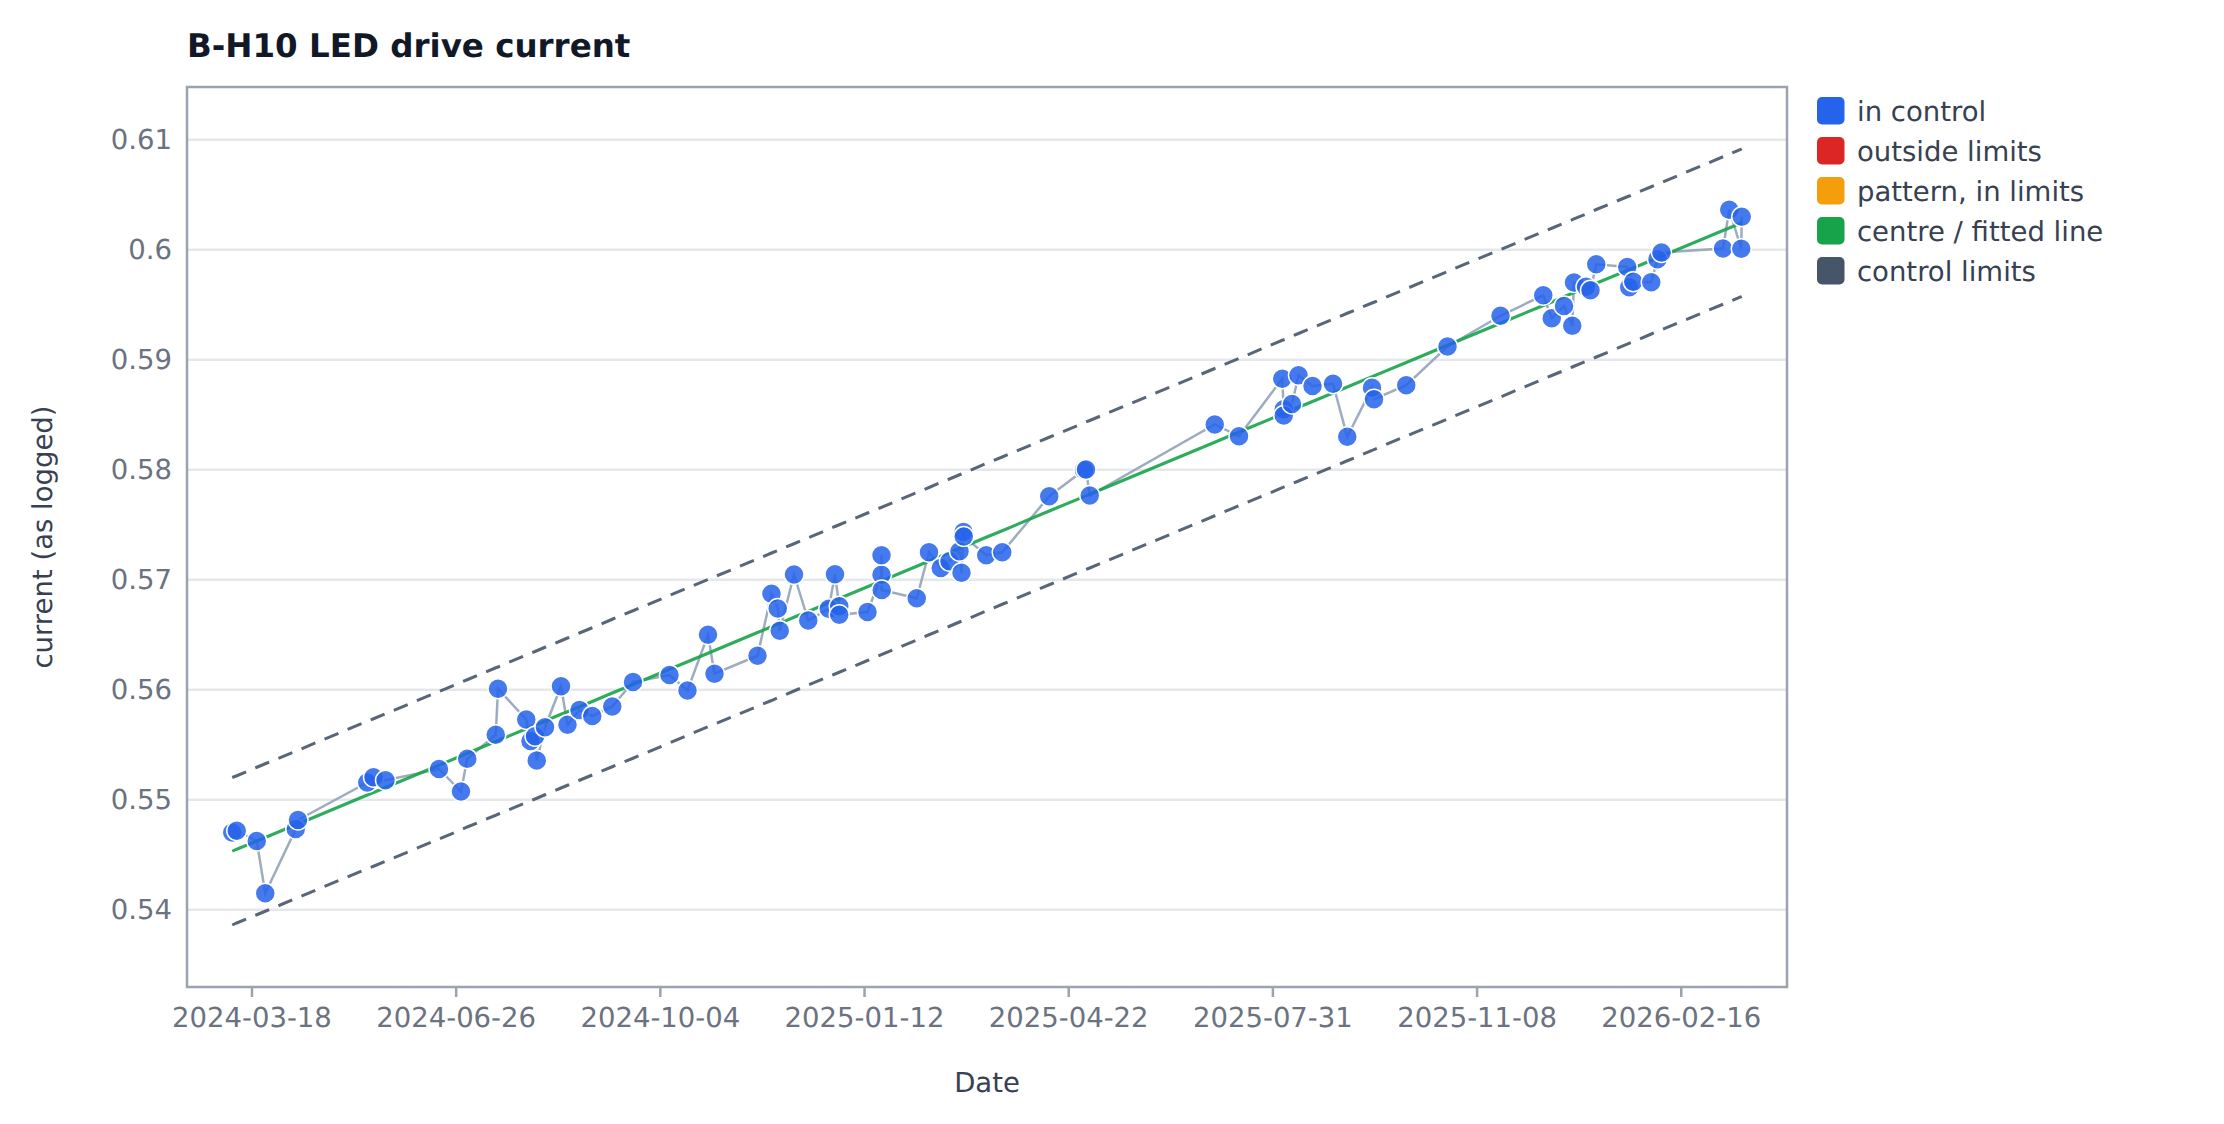
\includegraphics[width=\linewidth]{fig/cc_led_current_trend.png}\caption{B-H10 LED drive current}\end{subfigure}\hfill
\begin{subfigure}{0.49\linewidth}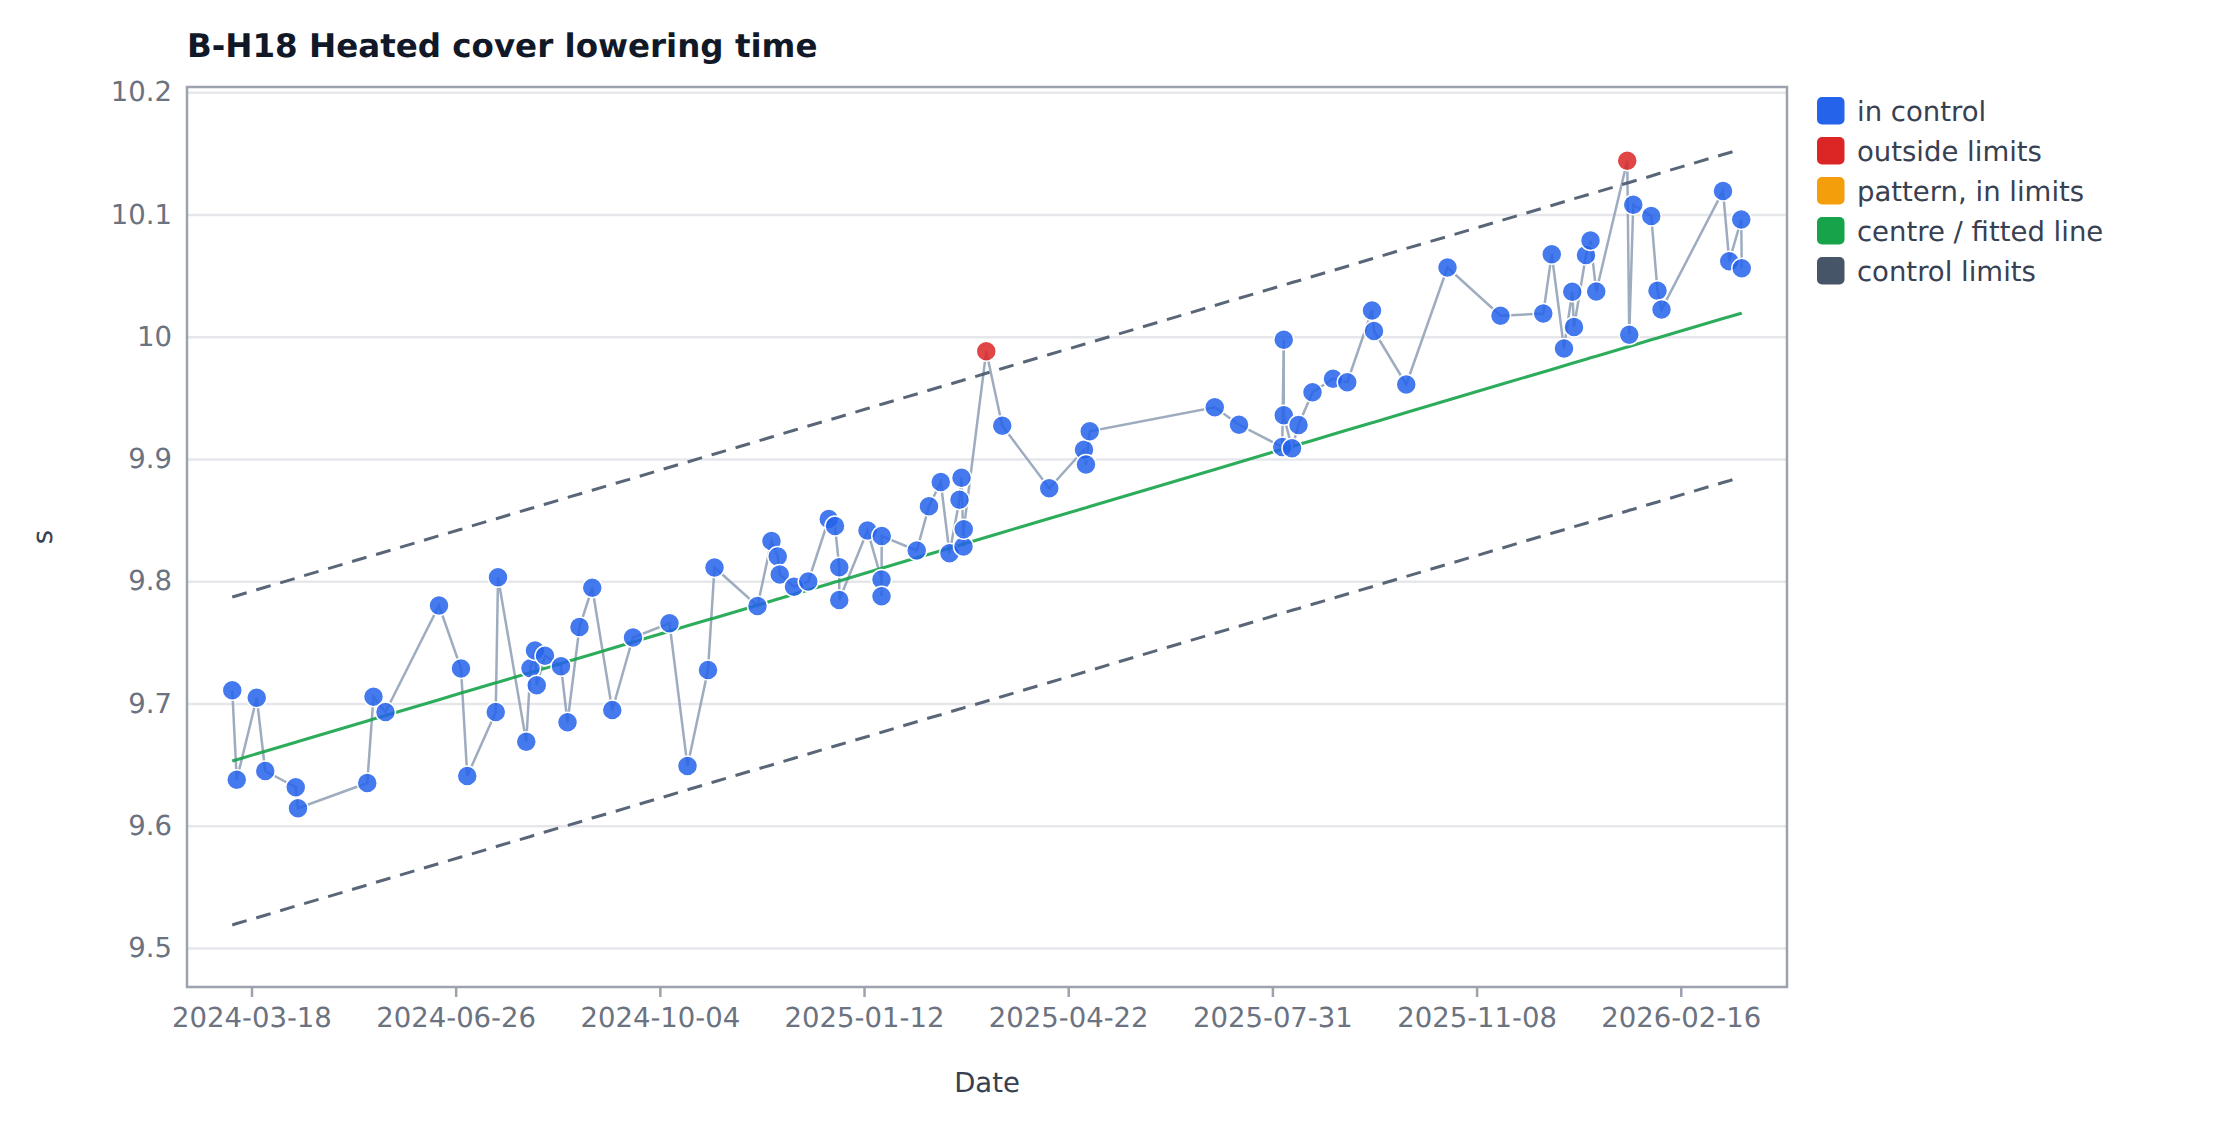
\includegraphics[width=\linewidth]{fig/cc_cover_down_trend.png}\caption{B-H18 heated cover lowering time}\end{subfigure}
\caption{\synthtag Trend charts, QS-DEMO-A: LED drive current and cover-motion time rise by construction. Departures from the fitted band prompt investigation; they do not establish a component failure.}\label{fig:qs_trends}
\end{figure}

\fig[0.9]{cc_heat_rate.png}{Trend chart, LC-DEMO-01, B-H1 peak heating rate against date. The baseline slope is not significant, so the centre line is flat; the planted service step is reported as a sustained shift (Figure~\ref{fig:shift}).}{heat}

\subsection{Sustained shifts and the proposed re-baseline}\label{sec:shift}
After a service, a firmware change or a block exchange the process moves to a new level; every later run then sits outside the
old limits and the chart would stay red indefinitely. \texttt{ccShift()} recognises this pattern — eight consecutive runs
outside on the same side and at least 70\,\% of the later runs on that side — and reports it as one finding: the date it
started, the level before and after, the number of runs since, and whether the new level is still inside the specification.
A button offers that date as the new \emph{baseline start}; nothing is re-baselined automatically, and the specification test
is independent of the control limits.

\par\medskip\noindent{\small\textbf{Listing}~\texttt{ccShift()}\hfill\textcolor{gray}{HTML lines 6074--6085}}\par\nopagebreak
\lstinputlisting[style=vstyle,language=JavaScript,firstnumber=6074]{code/ccShift.js}



\begin{figure}[htbp]\centering
\begin{subfigure}{0.49\linewidth}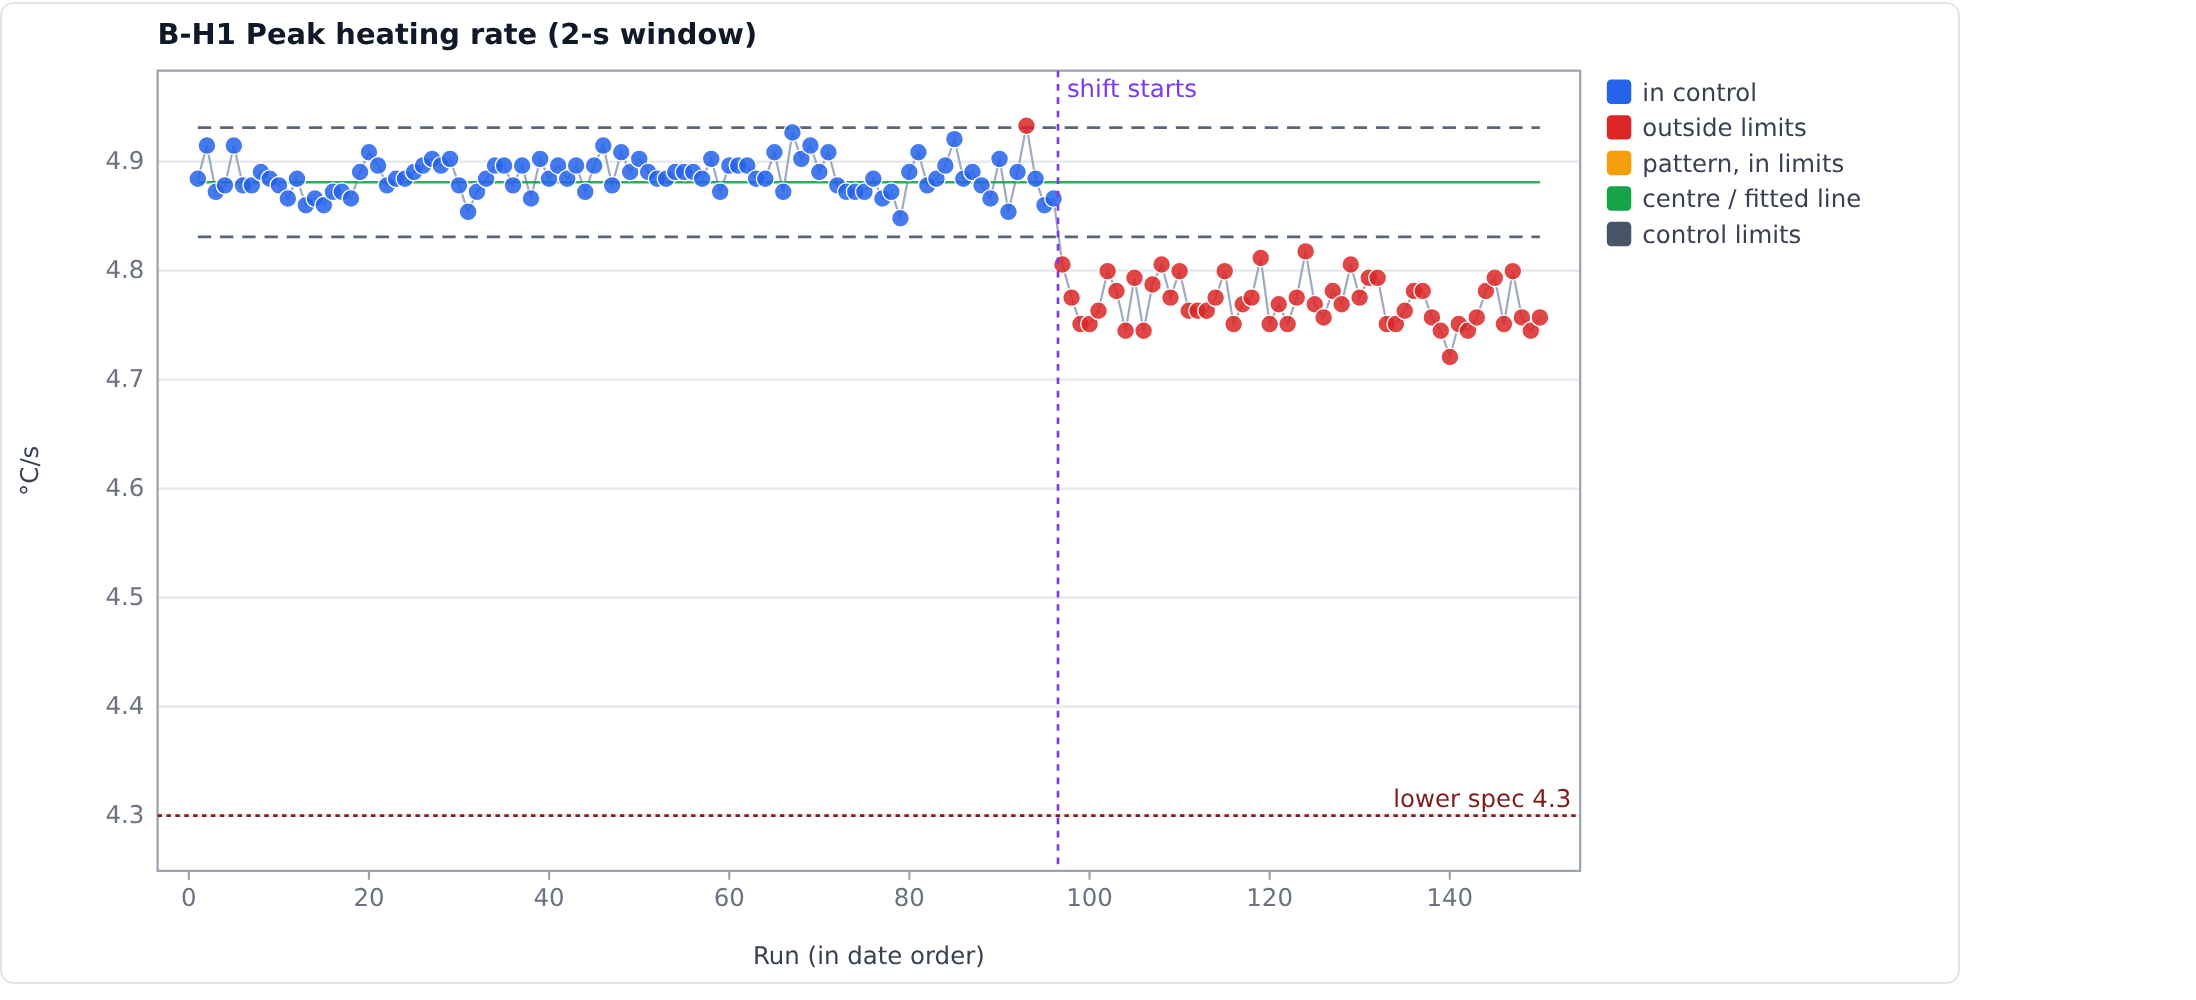
\includegraphics[width=\linewidth]{fig/cc_shift_heat_rate.png}\caption{shift detected, old baseline}\label{fig:shift_a}\end{subfigure}\hfill
\begin{subfigure}{0.49\linewidth}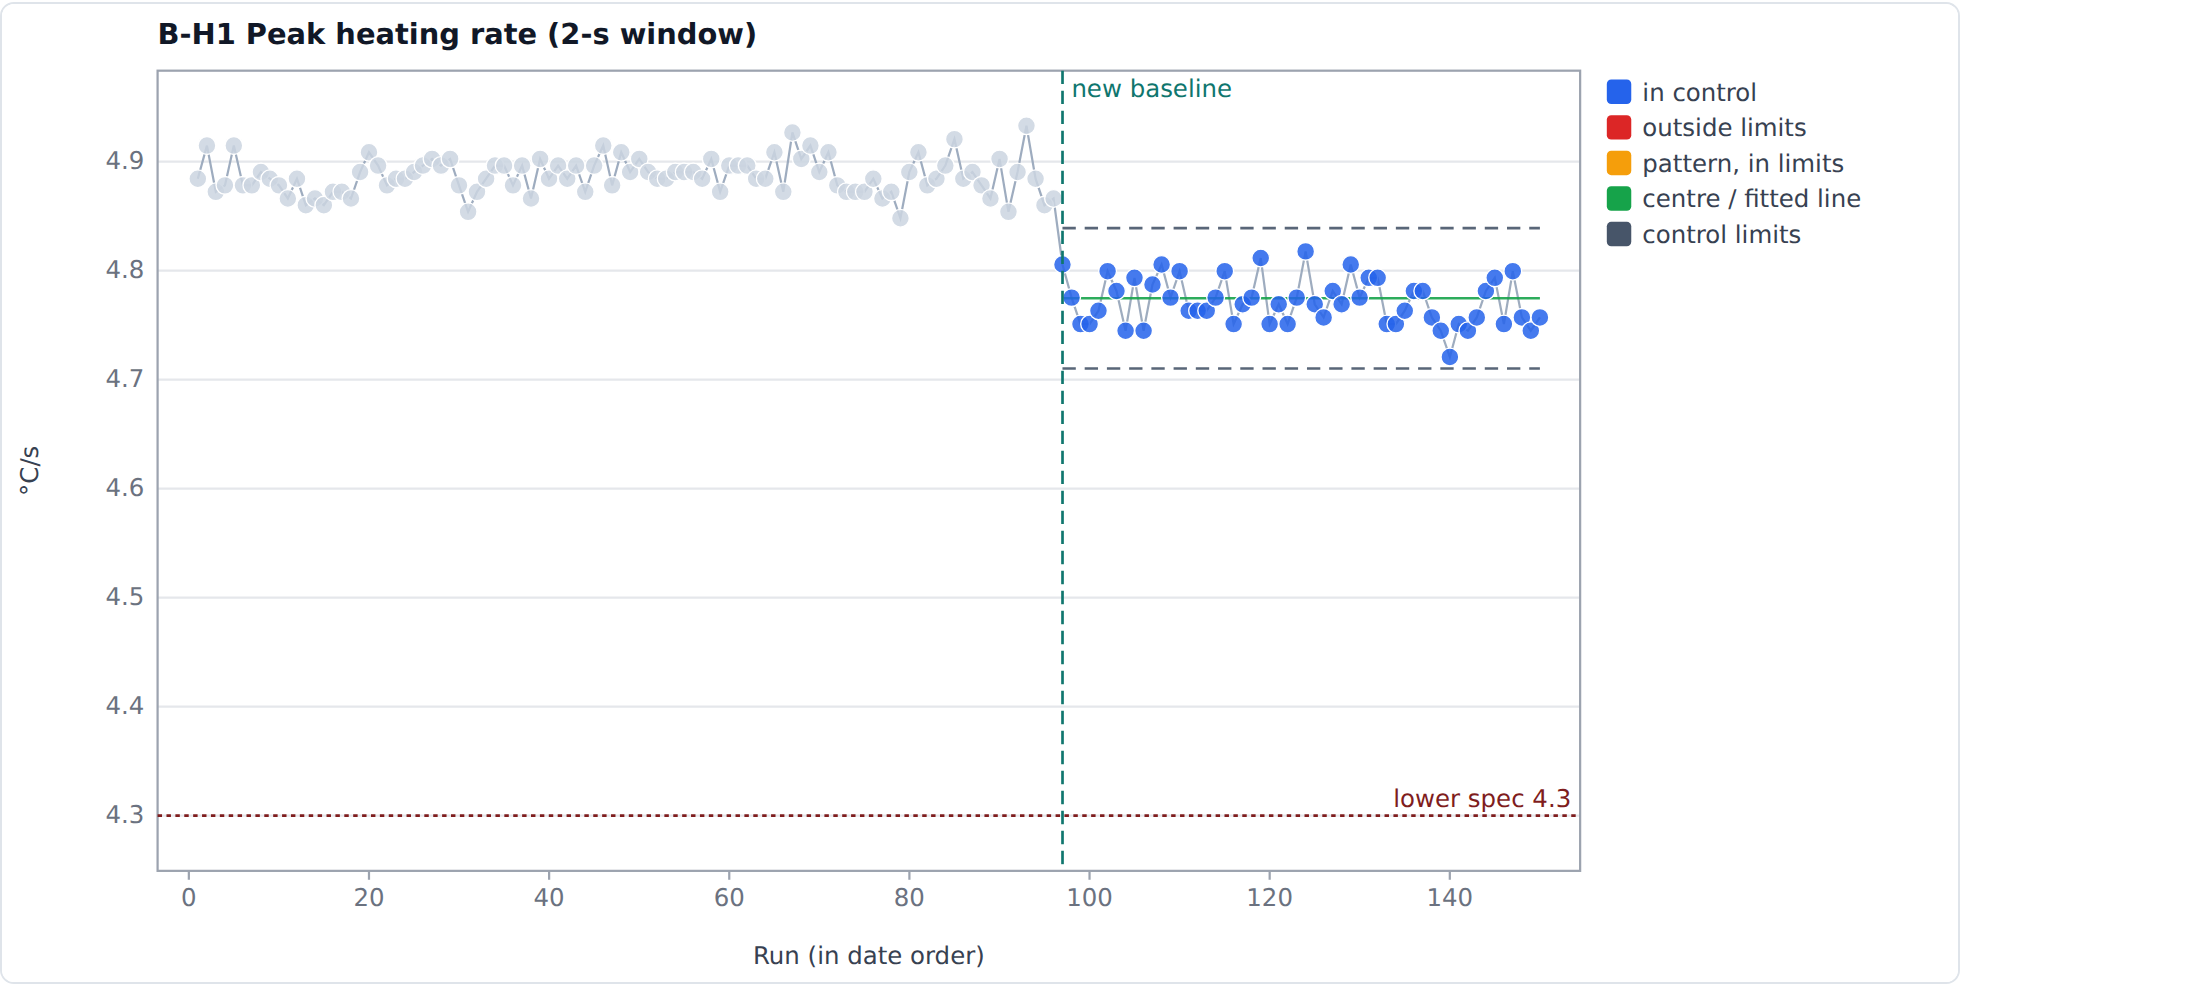
\includegraphics[width=\linewidth]{fig/cc_shift_heat_rate_rebased.png}\caption{after accepting the new baseline}\label{fig:shift_b}\end{subfigure}
\caption{\synthtag B-H1 peak heating rate, LC-DEMO-01, with the planted synthetic service step. (a) the shift is marked and
reported (4.88 $\to$ 4.77\,°C/s, still inside the 4.3\,°C/s specification); (b) with the baseline start set to that date the
earlier runs are grey and the limits describe the current level.}\label{fig:shift}
\end{figure}
\readingnote{A shift is a question about a cause, not a verdict on conformity: check the service record before accepting the
new baseline, and keep the specification comparison separate.}

\subsection{Three-way X̄–S chart}
For many readings per run (45 readings of the block temperature at the moment of reading, or all images of a run) the mean chart uses
\[ \bar{\bar x}\pm\max\!\Big(A_3(n)\,\bar S,\ 3\,\frac{\overline{MR}_{\bar x}}{1.128}\Big),\qquad \text{S chart: } B_4(n)\,\bar S,\quad c_4=\frac{4(n-1)}{4n-3}, \]
the three-way chart of Wheeler: with within-run limits alone ($A_3\bar S$) almost every run would alarm, because the run-to-run
variation is much larger than the variation inside a run.
\par\medskip\noindent{\small\textbf{Listing}~\texttt{ccXbarS()}\hfill\textcolor{gray}{HTML lines 6223--6234}}\par\nopagebreak
\lstinputlisting[style=vstyle,language=JavaScript,firstnumber=6223]{code/ccXbarS.js}


\fig[0.8]{cc_hold_temp_xbars.png}{X̄–S chart, LC-DEMO-01, B-H4 temperature at the moment of reading: the planted recalibration moves the offset from $-0.50$ to about $-0.40$\,°C; the within-run spread (S chart) stays unchanged.}{hold}

\subsection{Attribute charts: p, u, c}
\[ p:\ \bar p\pm3\sqrt{\bar p(1-\bar p)/n_i},\qquad u:\ \bar u\pm3\sqrt{\bar u/e_i},\qquad c:\ \bar c\pm3\sqrt{\bar c}. \]
\par\medskip\noindent{\small\textbf{Listing}~\texttt{ccP()}\hfill\textcolor{gray}{HTML lines 6209--6214}}\par\nopagebreak
\lstinputlisting[style=vstyle,language=JavaScript,firstnumber=6209]{code/ccP.js}


\par\medskip\noindent{\small\textbf{Listing}~\texttt{ccU()}\hfill\textcolor{gray}{HTML lines 6215--6218}}\par\nopagebreak
\lstinputlisting[style=vstyle,language=JavaScript,firstnumber=6215]{code/ccU.js}


\par\medskip\noindent{\small\textbf{Listing}~\texttt{ccC()}\hfill\textcolor{gray}{HTML lines 6219--6222}}\par\nopagebreak
\lstinputlisting[style=vstyle,language=JavaScript,firstnumber=6219]{code/ccC.js}


\fig[0.9]{cc_ntc_p.png}{p chart, B-M5 share of NTC / blank wells with a Cq. The limits widen and narrow with the number of NTC wells per run.}{ntcp}
\fig[0.9]{cc_copied.png}{c chart, B-O11 copied-data events: the planted copied curve in run 013 is the only event.}{copied}

\subsection{Funnel plot by operator}
Each operator is one point: rate against workload $n$, with 95\,\% and 99.8\,\% limits $p_0\pm1.96$ and $\pm3.09\sqrt{p_0(1-p_0)/n}$.
It compares people with different workloads fairly and is meant for training, not ranking.
\par\medskip\noindent{\small\textbf{Listing}~\texttt{ccFunnel()}\hfill\textcolor{gray}{HTML lines 6235--6241}}\par\nopagebreak
\lstinputlisting[style=vstyle,language=JavaScript,firstnumber=6235]{code/ccFunnel.js}


\fig[0.85]{cc_ntc_funnel.png}{Funnel plot, B-O5 selected negative-control stage by operator. Workload is shown, but assay and batch confounding are not adjusted.}{funnel}
\fig[0.9]{cc_rep_sd.png}{I chart coloured by operator, B-O1 replicate precision (pooled SD of replicates with Cq $<30$): the points of Analyst B sit higher.}{repsd}

\subsection{Transition times, lamp, exposure and processing delay}
\begin{figure}[htbp]\centering
\begin{subfigure}{0.49\linewidth}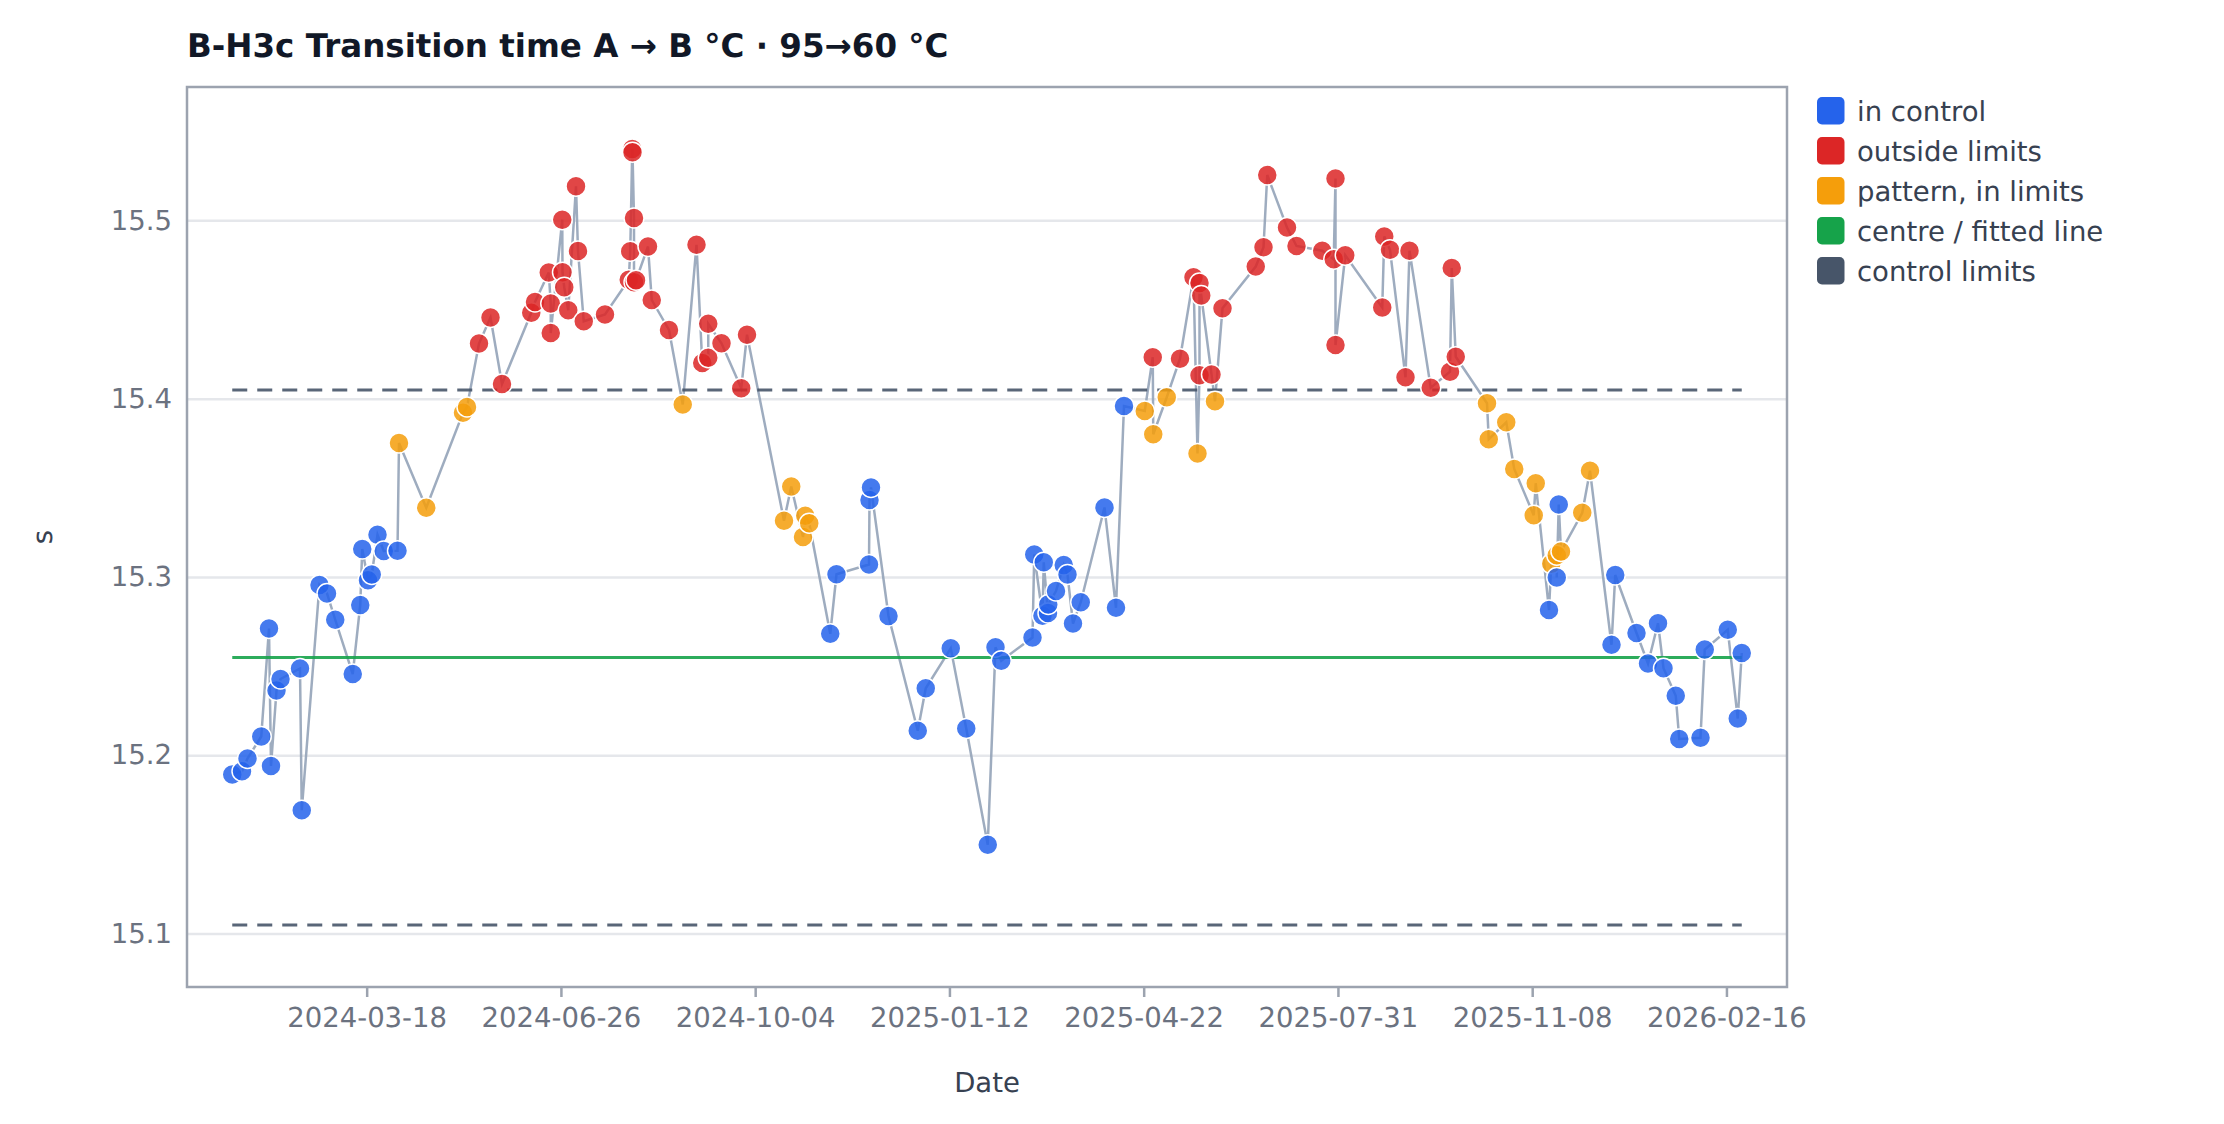
\includegraphics[width=\linewidth]{fig/cc_transition_95_60.png}\caption{95 $\to$ 60 °C}\end{subfigure}\hfill
\begin{subfigure}{0.49\linewidth}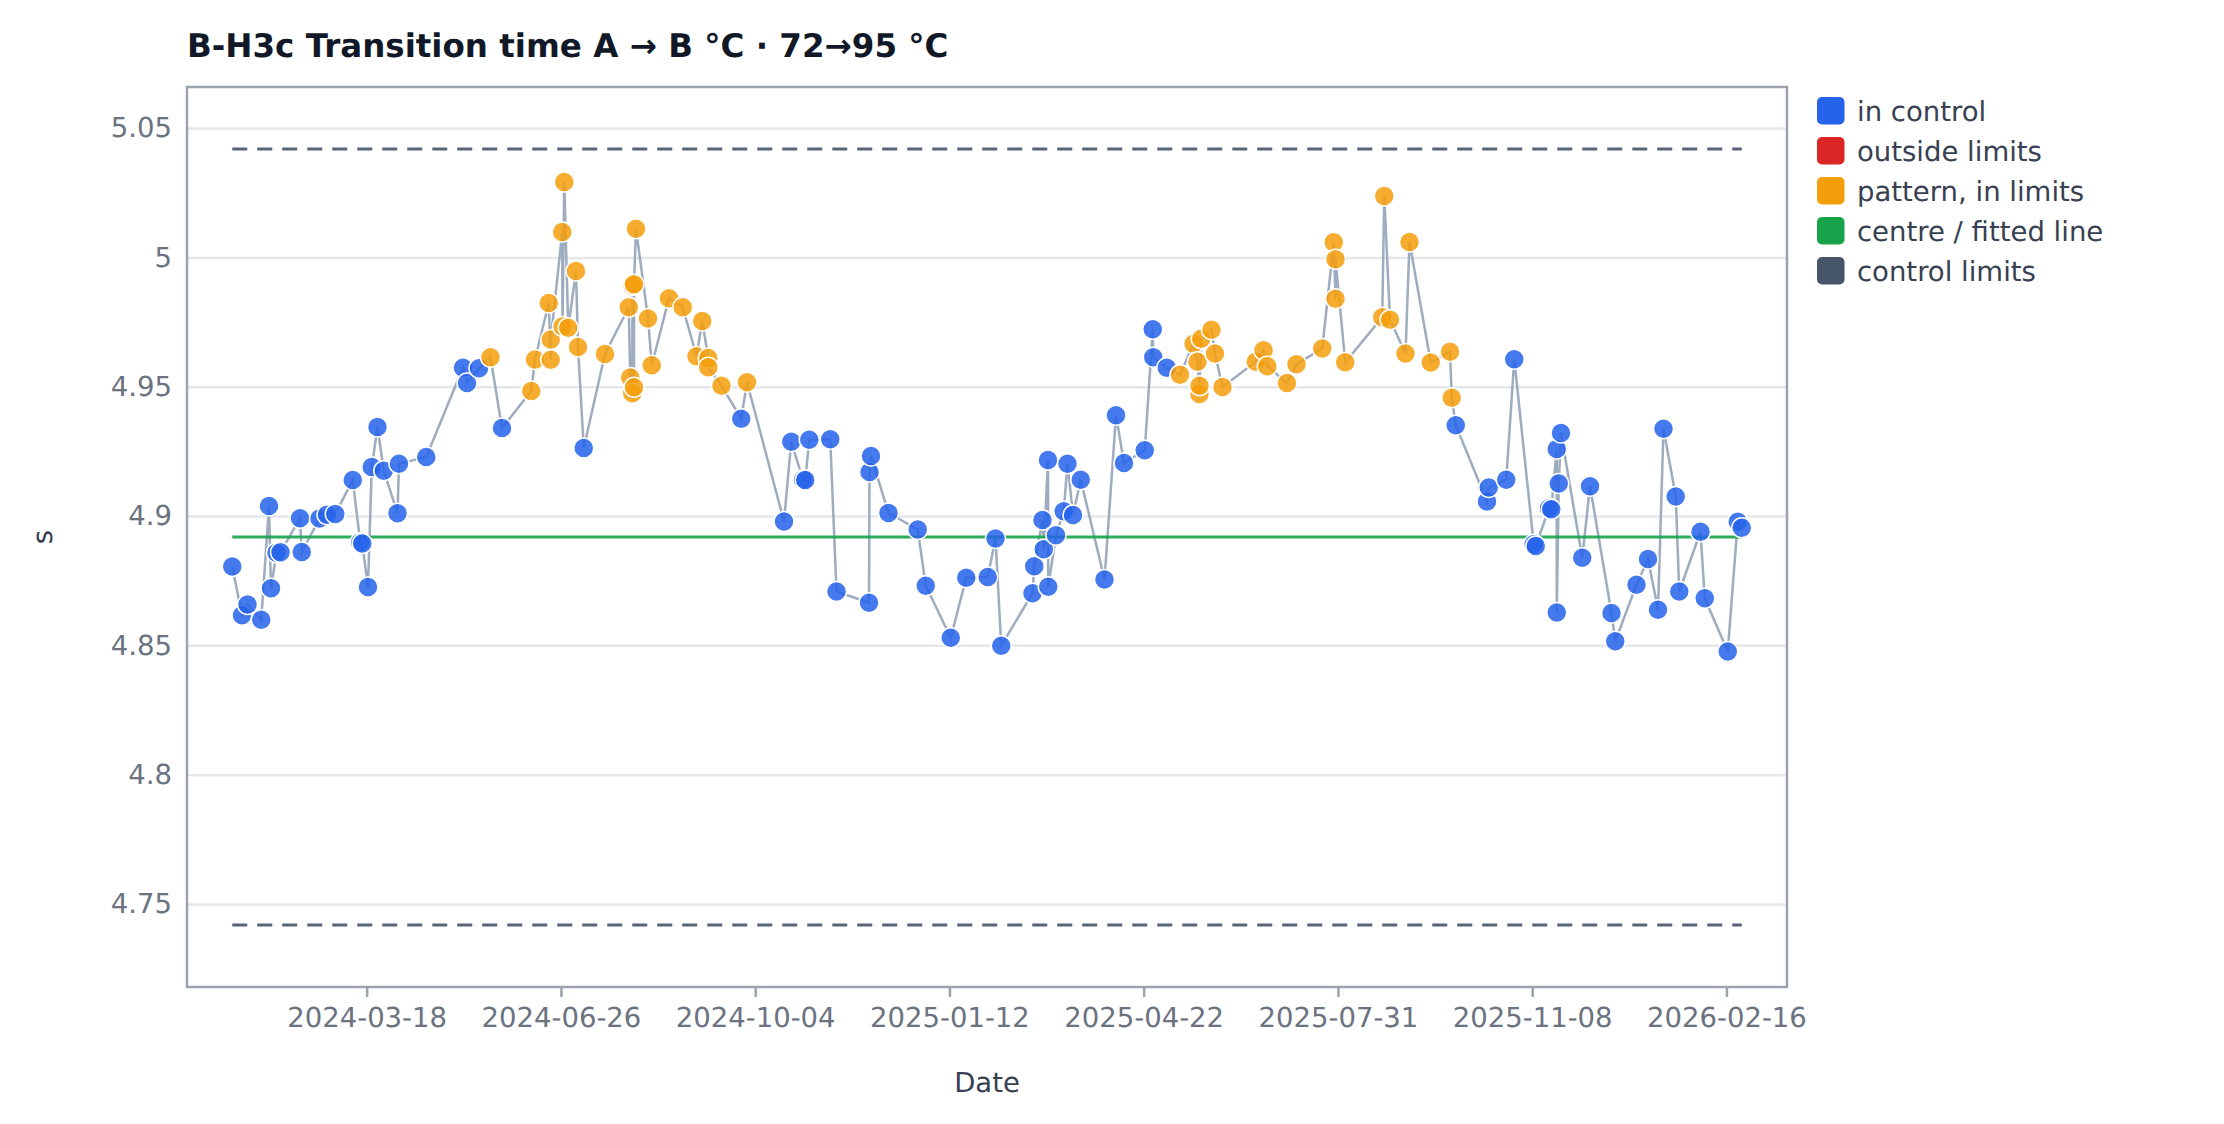
\includegraphics[width=\linewidth]{fig/cc_transition_72_95.png}\caption{72 $\to$ 95 °C}\end{subfigure}
\caption{\synthtag B-H3c transition times, LC-DEMO-01, against date. The history shows the planted seasonality (95\,$\to$\,60 longer in summer, 72\,$\to$\,95 longer in winter); in the most recent runs the cooling capacity drops below what the program asks for and 95\,$\to$\,60\,°C lengthens run after run.}\label{fig:trans}
\end{figure}
\fig[0.85]{cc_qs_transition_60_95.png}{B-H3c for QS-DEMO-A, 60 $\to$ 95 °C (1-s modelled sample temperature, interpolated crossings).}{qs_trans}
\begin{figure}[htbp]\centering
\begin{subfigure}{0.49\linewidth}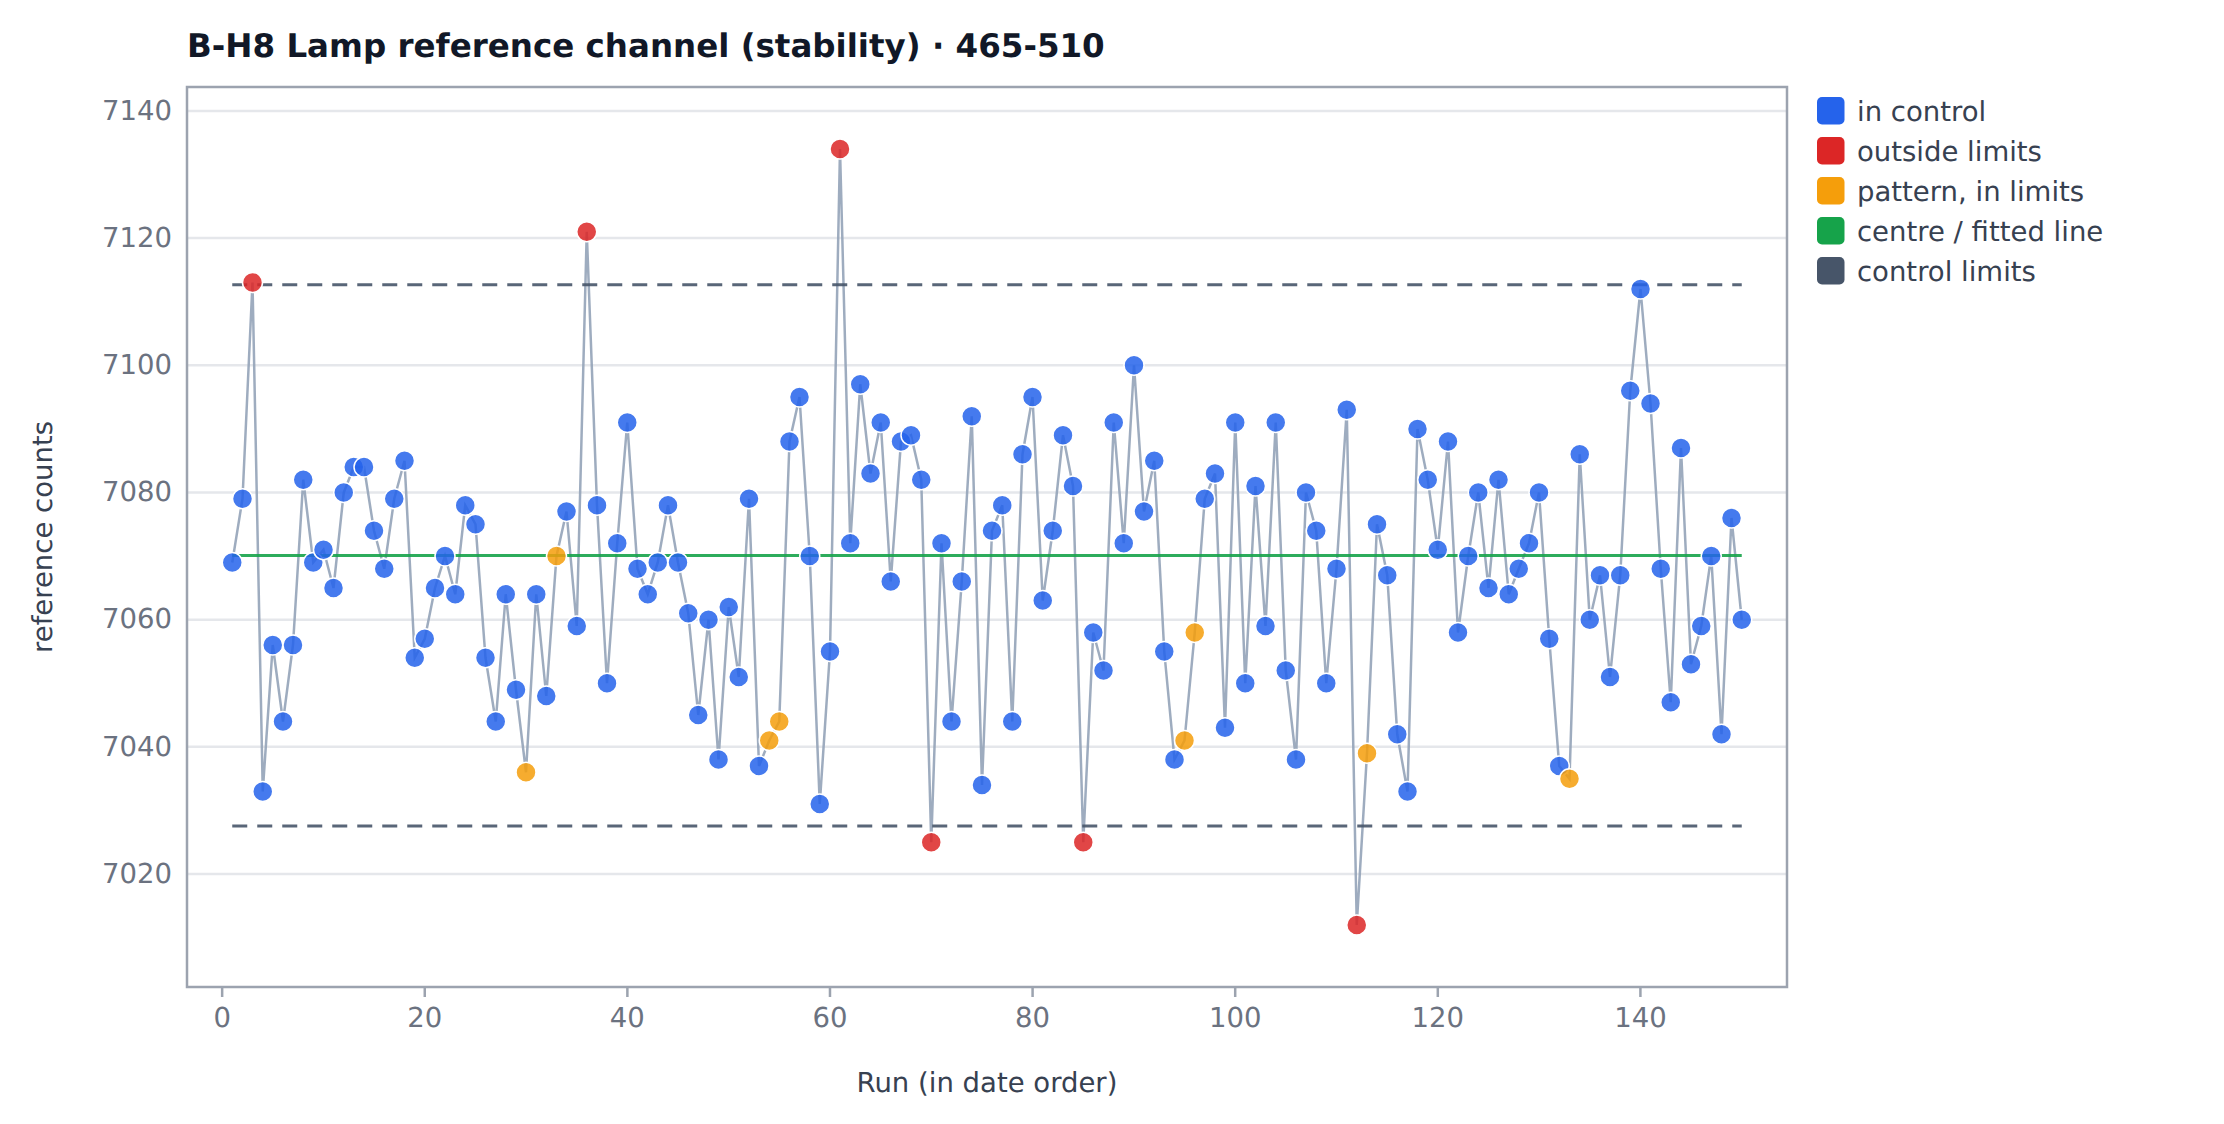
\includegraphics[width=\linewidth]{fig/cc_lamp_ref.png}\caption{B-H8 lamp reference channel 465-510}\end{subfigure}\hfill
\begin{subfigure}{0.49\linewidth}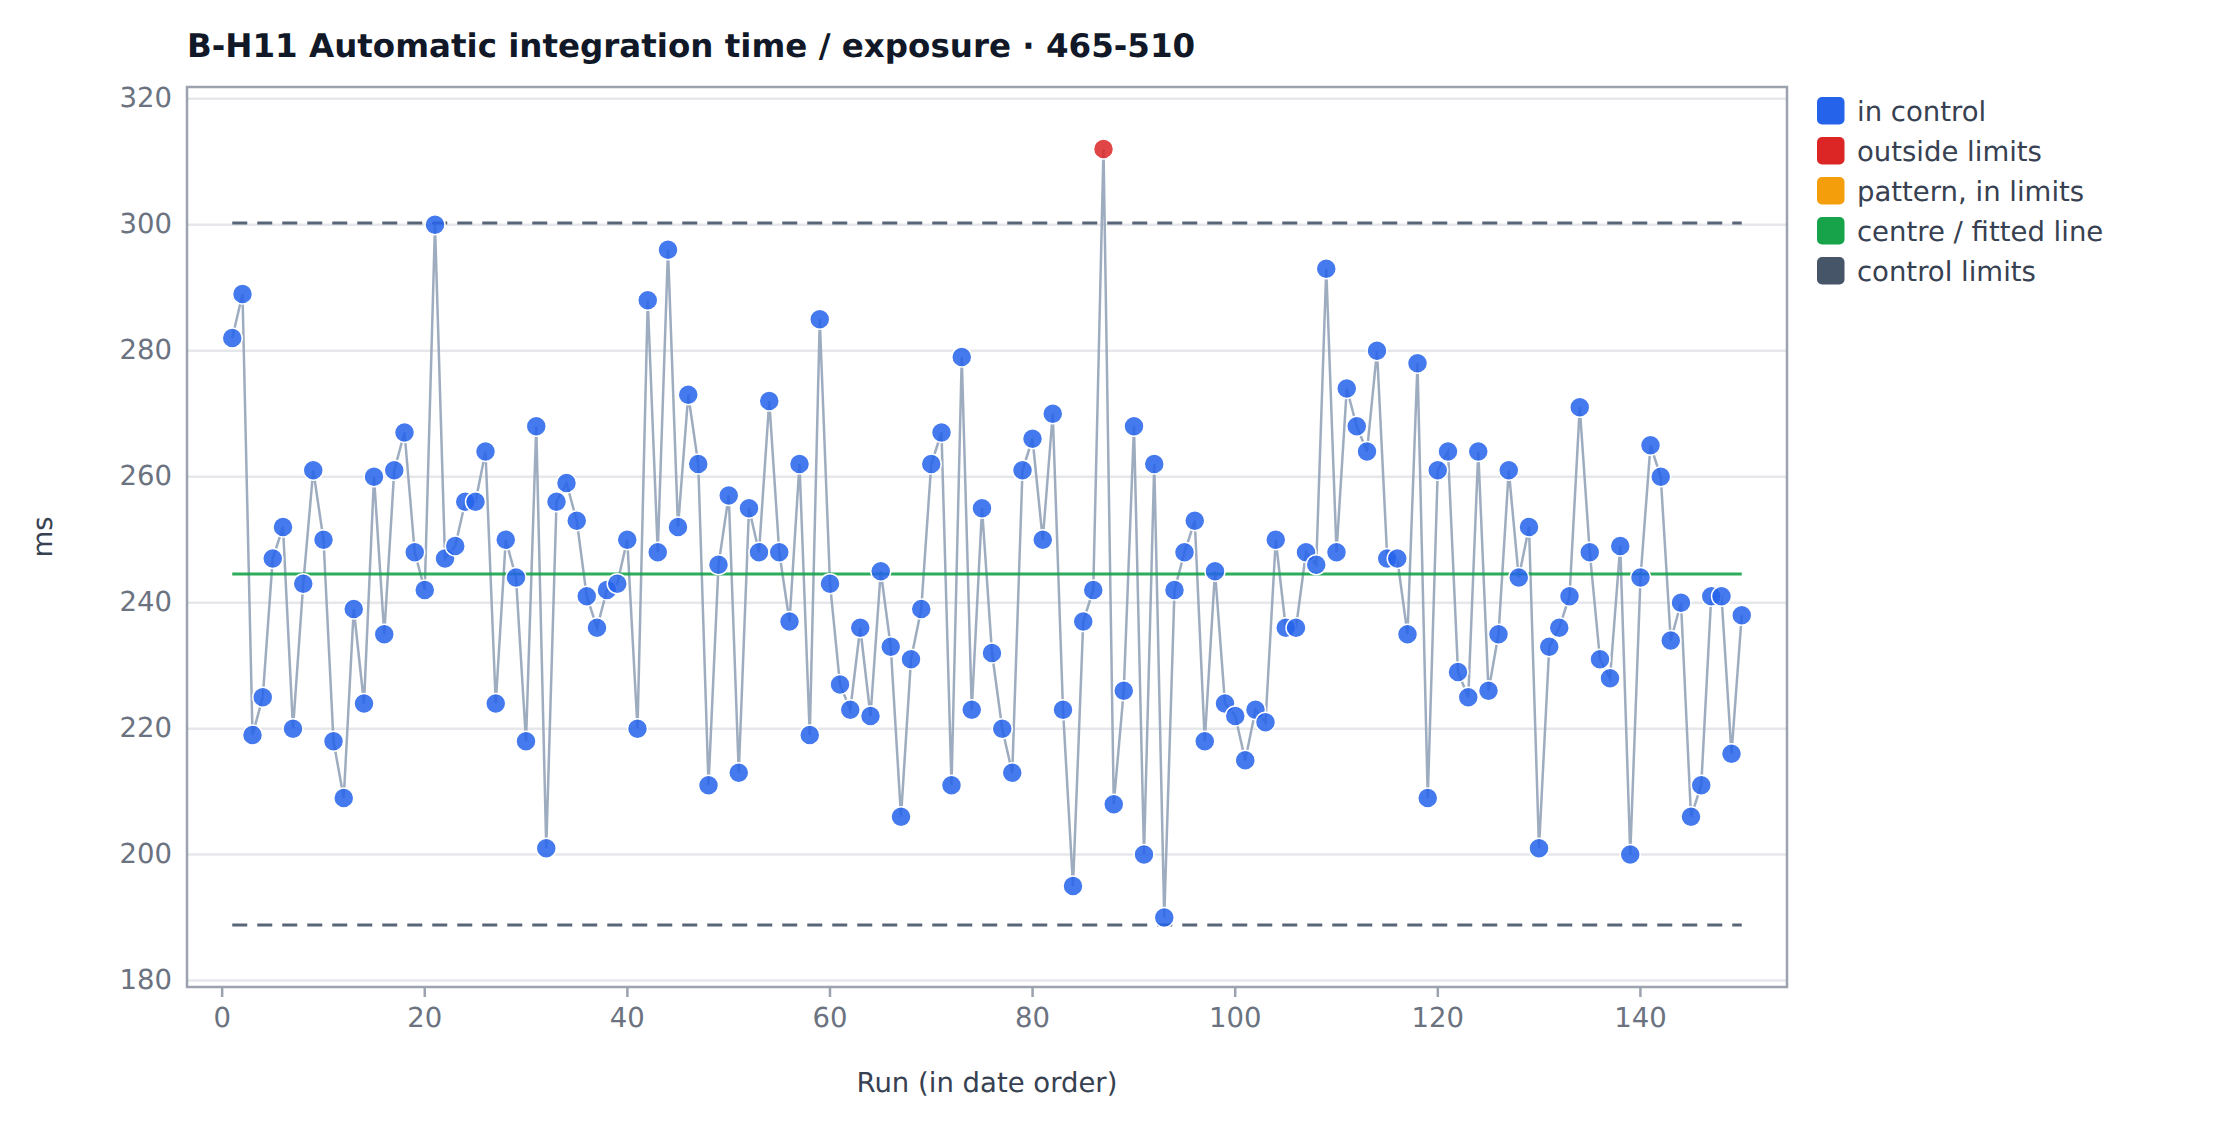
\includegraphics[width=\linewidth]{fig/cc_exposure.png}\caption{B-H11 automatic integration time 465-510}\end{subfigure}
\caption{\synthtag .ixo instrument optics: the lamp reference is regulated and stays flat; the exposure rises slowly as the synthetic optics lose light.}\label{fig:optics}
\end{figure}
\fig[0.9]{cc_edit_delay.png}{A-S4 run end $\to$ last change (log$_{10}$ hours): the planted late change of run 018 (410\,h) stands out.}{editdelay}
\fig[0.9]{cc_cmd_rt.png}{B-S1 reply time of the .eds instrument's embedded computer to the PC software (95th percentile per run).}{cmdrt}

\section{From chart definition to status}
\texttt{ccCompute()} selects the rows that carry the metric, applies the baseline date and the resolution floor, calls the
chart function and adds the specification limits; \texttt{ccStatus()} turns the result into the tile status.

\par\medskip\noindent{\small\textbf{Listing}~\texttt{CC\_GROUPS and the first entries of CC\_CHARTS}\hfill\textcolor{gray}{HTML lines 5940--5954}}\par\nopagebreak
\lstinputlisting[style=vstyle,language=JavaScript,firstnumber=5940]{code/cc_charts_head.js}


\par\medskip\noindent{\small\textbf{Listing}~\texttt{CC\_CHARTS entry B-H3c (transition time)}\hfill\textcolor{gray}{HTML lines 5963--5966}}\par\nopagebreak
\lstinputlisting[style=vstyle,language=JavaScript,firstnumber=5963]{code/cc_transition_def.js}


\par\medskip\noindent{\small\textbf{Listing}~\texttt{ccSpec()}\hfill\textcolor{gray}{HTML lines 6372--6377}}\par\nopagebreak
\lstinputlisting[style=vstyle,language=JavaScript,firstnumber=6372]{code/ccSpec.js}


\par\medskip\noindent{\small\textbf{Listing}~\texttt{ccXAxis()}\hfill\textcolor{gray}{HTML lines 6365--6371}}\par\nopagebreak
\lstinputlisting[style=vstyle,language=JavaScript,firstnumber=6365]{code/ccXAxis.js}


\par\medskip\noindent{\small\textbf{Listing}~\texttt{ccCompute()}\hfill\textcolor{gray}{HTML lines 6378--6428}}\par\nopagebreak
\lstinputlisting[style=vstyle,language=JavaScript,firstnumber=6378]{code/ccCompute.js}


\par\medskip\noindent{\small\textbf{Listing}~\texttt{ccStatus()}\hfill\textcolor{gray}{HTML lines 6444--6469}}\par\nopagebreak
\lstinputlisting[style=vstyle,language=JavaScript,firstnumber=6444]{code/ccStatus.js}



\section{The chart page and its settings}
\figui[0.9]{ui_chart_page_cool.png}{Chart page of B-H2: chart, status line with the forecast, \emph{How to read it}, the meaning of a result below and above the limits, and the settings of this chart.}{ui_chart_page}

Every chart has two texts that say what a result \textbf{below the lower limit} and \textbf{above the upper limit} means and
what to check first; the alarm table marks each alarm as ▼ below or ▲ above. Control-chart alarms stay in this panel so
quality review is reserved for file, timeline, result and interpretation evidence.

\figui{ui_limit_texts.png}{The two interpretation boxes of a chart page.}{ui_limits}
\par\medskip\noindent{\small\textbf{Listing}~\texttt{CC\_LIMIT\_TEXT — first entries (one per chart)}\hfill\textcolor{gray}{HTML lines 6244--6249}}\par\nopagebreak
\lstinputlisting[style=vstyle,language=JavaScript,firstnumber=6244]{code/cc_limit_text.js}


\par\medskip\noindent{\small\textbf{Listing}~\texttt{ccAlarmDir()}\hfill\textcolor{gray}{HTML lines 6308--6314}}\par\nopagebreak
\lstinputlisting[style=vstyle,language=JavaScript,firstnumber=6308]{code/ccAlarmDir.js}



The settings are stored in the SOP profile under \texttt{controlCharts}, so they are versioned and covered by the profile's
SHA-256 like any other rule (Chapter~\ref{ch:sop}).

\figui{ui_chart_settings.png}{Settings of a chart: alarm action, baseline runs, baseline start date (after a repair or service), specification limits, warning horizon and how the wear line is fitted.}{ui_settings}
\par\medskip\noindent{\small\textbf{Listing}~\texttt{CC\_DEFAULT\_CFG()}\hfill\textcolor{gray}{HTML lines 6131--6132}}\par\nopagebreak
\lstinputlisting[style=vstyle,language=JavaScript,firstnumber=6131]{code/CC_DEFAULT_CFG.js}


\par\medskip\noindent{\small\textbf{Listing}~\texttt{ccCfg()}\hfill\textcolor{gray}{HTML lines 6136--6137}}\par\nopagebreak
\lstinputlisting[style=vstyle,language=JavaScript,firstnumber=6136]{code/ccCfg.js}


\par\medskip\noindent{\small\textbf{Listing}~\texttt{ccSetCfg()}\hfill\textcolor{gray}{HTML lines 6138--6139}}\par\nopagebreak
\lstinputlisting[style=vstyle,language=JavaScript,firstnumber=6138]{code/ccSetCfg.js}



\section{Alarms in the control panel}
The panel summary counts alarm points for the selected instrument and lists them by chart. These are monitoring signals,
not duplicate forensic findings. The chart CSV and SVG exports retain the full alarm detail.
\par\medskip\noindent{\small\textbf{Listing}~\texttt{ccEvents()}\hfill\textcolor{gray}{HTML lines 6777--6788}}\par\nopagebreak
\lstinputlisting[style=vstyle,language=JavaScript,firstnumber=6777]{code/ccEvents.js}



\section{All control charts of all instruments in one ZIP}
The button \emph{All control charts, all instruments (ZIP)} writes, for every instrument, every chart (and every channel,
target or transition) as SVG and CSV (optionally PNG), a summary table and the instrument history:

\begin{lstlisting}[style=vstyle,language=text, numbers=left,firstnumber=1]
control_charts_all_instruments_<date>.zip
├── README.txt            profile, SHA-256, protocol filter, one line per instrument
├── sop_profile.json
├── LC_LC-DEMO-01/        86 files
│   ├── 00_summary.csv    status of every chart on the latest run
│   ├── B-H2_cool_rate.svg / .csv
│   ├── B-H3c_transition_95-to-60.svg / .csv
│   ├── B-H4_hold_temp.svg, B-H4_hold_temp_S-chart.svg, .csv
│   ├── … one file pair per chart and variant
│   └── history.json / history.csv
├── LC_LC-DEMO-02/  QS_QS-DEMO-A/  QS_QS-DEMO-B/
\end{lstlisting}
The synthetic data set gives 407 files in four folders.

{\footnotesize
\begin{longtable}{@{}lllllll@{}}
\toprule \textbf{Column 1} & \textbf{Column 2} & \textbf{Column 3} & \textbf{Column 4} & \textbf{Column 5} & \textbf{Column 6} & \textbf{Column 7} \\\midrule\endfirsthead
\toprule \textbf{Column 1} & \textbf{Column 2} & \textbf{Column 3} & \textbf{Column 4} & \textbf{Column 5} & \textbf{Column 6} & \textbf{Column 7} \\\midrule\endhead
A-H4 & Run duration &  & alarm & 97.597 & 36 & 8 on one side \\\hline
A-M1 & Positive control … & 35S | DEMO LOD 01… & alarm & 32.125 & 19 & 10-x \\\hline
B-H1 & Peak heating rate… &  & alarm & 4.780 & 127 & off the trend lin… \\\hline
B-H2 & Peak cooling rate… &  & alarm & 2.238 & 15 & off the trend lin… \\\hline
B-H3 & Overshoot at the … &  & alarm & 6.100 & 113 & downward shift (C… \\\hline
B-H3b & Settling time at … &  & alarm & 5.330 & 152 & beyond 3σ, 2 of 3… \\\hline
B-H3c & Transition time A… & 95→60 °C & alarm & 15.292 & 124 & beyond 3σ, 2 of 3… \\\hline
B-H3c & Transition time A… & 60→72 °C & alarm & 2.330 & 37 & 8 on one side \\\hline
B-H3c & Transition time A… & 72→95 °C & alarm & 5.797 & 108 & 8 on one side \\\hline
B-H3c & Transition time A… & 72→40 °C & alarm & 13.965 & 27 & 4 of 5 beyond 1σ,… \\\hline
B-H4 & Temperature at th… &  & alarm & -0.412 & 87 & mean beyond limit \\\hline
B-O1 & Replicate precisi… &  & alarm & 0.718 & 33 & beyond 3σ, 2 of 3… \\\hline
\bottomrule
\end{longtable}}


\par\medskip\noindent{\small\textbf{Listing}~\texttt{ccChartRows()}\hfill\textcolor{gray}{HTML lines 6672--6679}}\par\nopagebreak
\lstinputlisting[style=vstyle,language=JavaScript,firstnumber=6672]{code/ccChartRows.js}


\par\medskip\noindent{\small\textbf{Listing}~\texttt{ccZipAll()}\hfill\textcolor{gray}{HTML lines 6689--6737}}\par\nopagebreak
\lstinputlisting[style=vstyle,language=JavaScript,firstnumber=6689]{code/ccZipAll.js}



\figui[0.82]{ui_panel_qsa.png}{Control panel for the synthetic .eds instrument \texttt{QS-DEMO-A}: the .eds instrument-only charts (LED, zones, heat sink, cover, filter wheel, camera, embedded computer, calibrations) appear here.}{ui_panel_qsa}


